% igs2ejournalguide.tex
%DIF LATEXDIFF DIFFERENCE FILE
%DIF DEL WinterBalance.tex          Tue Jan  2 09:55:36 2018
%DIF ADD UncertaintyWB_Review.tex   Mon Mar  5 09:43:19 2018
% v4.00 3-sept-2015

\NeedsTeXFormat{LaTeX2e}

% check that the math fits the two-column format:
%DIF 7c7
%DIF < \documentclass[twocolumn, letterpaper]{igs}
%DIF -------
%\documentclass[twocolumn, letterpaper]{igs} %DIF > 
%DIF -------

% but use this version when submitting your article:
%DIF 10c10
%DIF < %\documentclass[review,oneside, letterpaper]{igs}
%DIF -------
\documentclass[review,oneside, letterpaper]{igs} %DIF > 
%DIF -------

  \usepackage{igsnatbib}
  \usepackage{lmodern}
\usepackage{amsmath,amssymb,amsthm}
\usepackage{wrapfig}
\usepackage{enumitem}
\usepackage{multirow}
\usepackage{tabularx}
\usepackage{booktabs}
\usepackage{lscape}
\usepackage{color}

\newcolumntype{C}{>{\centering\arraybackslash}X}
\renewcommand{\tabularxcolumn}[1]{m{#1}}%


% check if we are compiling under latex or pdflatex
  \ifx\pdftexversion\undefined
    \usepackage[dvips]{graphicx}
  \else
    \usepackage[pdftex]{graphicx}
    \usepackage{epstopdf}
    \epstopdfsetup{suffix=}
  \fi
%DIF PREAMBLE EXTENSION ADDED BY LATEXDIFF
%DIF UNDERLINE PREAMBLE %DIF PREAMBLE
\RequirePackage[normalem]{ulem} %DIF PREAMBLE
\RequirePackage{color}\definecolor{RED}{rgb}{1,0,0}\definecolor{BLUE}{rgb}{0,0,1} %DIF PREAMBLE
\providecommand{\DIFadd}[1]{{\protect\color{blue}\uwave{#1}}} %DIF PREAMBLE
\providecommand{\DIFdel}[1]{{\protect\color{red}\sout{#1}}}                      %DIF PREAMBLE
%DIF SAFE PREAMBLE %DIF PREAMBLE
\providecommand{\DIFaddbegin}{} %DIF PREAMBLE
\providecommand{\DIFaddend}{} %DIF PREAMBLE
\providecommand{\DIFdelbegin}{} %DIF PREAMBLE
\providecommand{\DIFdelend}{} %DIF PREAMBLE
%DIF FLOATSAFE PREAMBLE %DIF PREAMBLE
\providecommand{\DIFaddFL}[1]{\DIFadd{#1}} %DIF PREAMBLE
\providecommand{\DIFdelFL}[1]{\DIFdel{#1}} %DIF PREAMBLE
\providecommand{\DIFaddbeginFL}{} %DIF PREAMBLE
\providecommand{\DIFaddendFL}{} %DIF PREAMBLE
\providecommand{\DIFdelbeginFL}{} %DIF PREAMBLE
\providecommand{\DIFdelendFL}{} %DIF PREAMBLE
\newcommand{\DIFscaledelfig}{0.5}
%DIF HIGHLIGHTGRAPHICS PREAMBLE %DIF PREAMBLE
\RequirePackage{settobox} %DIF PREAMBLE
\RequirePackage{letltxmacro} %DIF PREAMBLE
\newsavebox{\DIFdelgraphicsbox} %DIF PREAMBLE
\newlength{\DIFdelgraphicswidth} %DIF PREAMBLE
\newlength{\DIFdelgraphicsheight} %DIF PREAMBLE
% store original definition of \includegraphics %DIF PREAMBLE
\LetLtxMacro{\DIFOincludegraphics}{\includegraphics} %DIF PREAMBLE
\newcommand{\DIFaddincludegraphics}[2][]{{\color{blue}\fbox{\DIFOincludegraphics[#1]{#2}}}} %DIF PREAMBLE
\newcommand{\DIFdelincludegraphics}[2][]{% %DIF PREAMBLE
\sbox{\DIFdelgraphicsbox}{\DIFOincludegraphics[#1]{#2}}% %DIF PREAMBLE
\settoboxwidth{\DIFdelgraphicswidth}{\DIFdelgraphicsbox} %DIF PREAMBLE
\settoboxtotalheight{\DIFdelgraphicsheight}{\DIFdelgraphicsbox} %DIF PREAMBLE
\scalebox{\DIFscaledelfig}{% %DIF PREAMBLE
\parbox[b]{\DIFdelgraphicswidth}{\usebox{\DIFdelgraphicsbox}\\[-\baselineskip] \rule{\DIFdelgraphicswidth}{0em}}\llap{\resizebox{\DIFdelgraphicswidth}{\DIFdelgraphicsheight}{% %DIF PREAMBLE
\setlength{\unitlength}{\DIFdelgraphicswidth}% %DIF PREAMBLE
\begin{picture}(1,1)% %DIF PREAMBLE
\thicklines\linethickness{2pt} %DIF PREAMBLE
{\color[rgb]{1,0,0}\put(0,0){\framebox(1,1){}}}% %DIF PREAMBLE
{\color[rgb]{1,0,0}\put(0,0){\line( 1,1){1}}}% %DIF PREAMBLE
{\color[rgb]{1,0,0}\put(0,1){\line(1,-1){1}}}% %DIF PREAMBLE
\end{picture}% %DIF PREAMBLE
}\hspace*{3pt}}} %DIF PREAMBLE
} %DIF PREAMBLE
\LetLtxMacro{\DIFOaddbegin}{\DIFaddbegin} %DIF PREAMBLE
\LetLtxMacro{\DIFOaddend}{\DIFaddend} %DIF PREAMBLE
\LetLtxMacro{\DIFOdelbegin}{\DIFdelbegin} %DIF PREAMBLE
\LetLtxMacro{\DIFOdelend}{\DIFdelend} %DIF PREAMBLE
\DeclareRobustCommand{\DIFaddbegin}{\DIFOaddbegin \let\includegraphics\DIFaddincludegraphics} %DIF PREAMBLE
\DeclareRobustCommand{\DIFaddend}{\DIFOaddend \let\includegraphics\DIFOincludegraphics} %DIF PREAMBLE
\DeclareRobustCommand{\DIFdelbegin}{\DIFOdelbegin \let\includegraphics\DIFdelincludegraphics} %DIF PREAMBLE
\DeclareRobustCommand{\DIFdelend}{\DIFOaddend \let\includegraphics\DIFOincludegraphics} %DIF PREAMBLE
\LetLtxMacro{\DIFOaddbeginFL}{\DIFaddbeginFL} %DIF PREAMBLE
\LetLtxMacro{\DIFOaddendFL}{\DIFaddendFL} %DIF PREAMBLE
\LetLtxMacro{\DIFOdelbeginFL}{\DIFdelbeginFL} %DIF PREAMBLE
\LetLtxMacro{\DIFOdelendFL}{\DIFdelendFL} %DIF PREAMBLE
\DeclareRobustCommand{\DIFaddbeginFL}{\DIFOaddbeginFL \let\includegraphics\DIFaddincludegraphics} %DIF PREAMBLE
\DeclareRobustCommand{\DIFaddendFL}{\DIFOaddendFL \let\includegraphics\DIFOincludegraphics} %DIF PREAMBLE
\DeclareRobustCommand{\DIFdelbeginFL}{\DIFOdelbeginFL \let\includegraphics\DIFdelincludegraphics} %DIF PREAMBLE
\DeclareRobustCommand{\DIFdelendFL}{\DIFOaddendFL \let\includegraphics\DIFOincludegraphics} %DIF PREAMBLE
%DIF END PREAMBLE EXTENSION ADDED BY LATEXDIFF

\begin{document}

\title[Estimating winter balance and its uncertainty]{Estimating winter balance and its uncertainty from direct measurements of snow depth and density on alpine glaciers}

\author[Pulwicki and others]{Alexandra PULWICKI,$^1$
  Gwenn E. FLOWERS,$^1$ Valentina  RADI\'C,$^2$ \DIFaddbegin \DIFadd{Derek  BINGHAM$^3$}\DIFaddend }

\DIFdelbegin %DIFDELCMD < \affiliation{%
%DIFDELCMD < $^1$ Department of Earth Sciences, Faculty of Science, Simon Fraser University, Burnaby, BC, Canada\\
%DIFDELCMD < $^2$Department of Earth, Ocean and Atmospheric Sciences, Faculty of Science, University of British Columbia, Vancouver, BC, Canada\\
%DIFDELCMD <   Correspondence: Alexandra Pulwicki 
%DIFDELCMD <   $<$apulwick@sfu.ca$>$}
%DIFDELCMD < %%%
\DIFdelend \DIFaddbegin \affiliation{%
$^1$ Department of Earth Sciences, Faculty of Science, Simon Fraser University, Burnaby, BC, Canada\\
$^2$Department of Earth, Ocean and Atmospheric Sciences, Faculty of Science, University of British Columbia, Vancouver, BC, Canada\\
$^3$ Department of Statistics and Actuarial Science, Faculty of Science, Simon Fraser University, Burnaby, BC, Canada\\
  Correspondence: Alexandra Pulwicki 
  $<$apulwick@sfu.ca$>$}
\DIFaddend 


%%%%%%%%%%%%%%%%%%%%%%%%%%%%%%%%%
%	ABSTRACT
%%%%%%%%%%%%%%%%%%%%%%%%%%%%%%%%%

\DIFdelbegin %DIFDELCMD < \abstract{Accurately estimating winter surface mass balance on glaciers is central to assessing glacier health and predicting glacier runoff. However, measuring and modelling snow distribution is inherently difficult in mountainous terrain. Here we explore rigorous statistical methods of estimating winter balance and its uncertainty from multiscale measurements of snow depth and density. In May 2016 we collected over 9000 manual measurements of snow depth across three glaciers in the St. Elias Mountains, Yukon, Canada. Linear regression, combined with cross correlation and Bayesian model averaging, as well as simple kriging are used to interpolate point-scale values to glacier-wide estimates of winter balance. Elevation and a wind-redistribution parameter exhibit the highest correlations with winter balance, but the relationship varies considerably between glaciers. A Monte Carlo analysis reveals that the interpolation itself introduces more uncertainty than the assignment of snow density or the representation of grid-scale variability. For our study glaciers, the winter balance uncertainty from all assessed sources ranges from 0.03\,m\,w.e. (8\%) to 0.15\,m\,w.e. (54\%). Despite the challenges associated with estimating winter balance, our results are consistent with a regional-scale winter-balance gradient. }
%DIFDELCMD < %%%
\DIFdelend \DIFaddbegin \abstract{Accurately estimating winter surface mass balance on glaciers is central to assessing glacier health and predicting glacier runoff. However, measuring and modelling snow distribution is inherently difficult in mountainous terrain. Here we explore rigorous statistical methods of estimating winter balance and its uncertainty from multiscale measurements of snow depth and density. In May 2016 we collected over 9000 manual measurements of snow depth across three glaciers in the St. Elias Mountains, Yukon, Canada. Linear regression, combined with cross correlation and Bayesian model averaging, as well as ordinary kriging are used to interpolate point-scale values to glacier-wide estimates of winter balance. Elevation and a wind-redistribution parameter exhibit the highest correlations with winter balance, but the relationship varies considerably between glaciers. A Monte Carlo analysis reveals that the interpolation itself introduces more uncertainty than the assignment of snow density or the representation of grid-scale variability. For our study glaciers, the winter balance uncertainty from all assessed sources ranges from 0.03\,m\,w.e. (8\%) to 0.15\,m\,w.e. (54\%). Despite the challenges associated with estimating winter balance, our results are consistent with a regional-scale winter-balance gradient. }
\DIFaddend \maketitle



%%%%%%%%%%%%%%%%%%%%%%%%%%%%%%%%%
%	INTRODUCTION
%%%%%%%%%%%%%%%%%%%%%%%%%%%%%%%%%
\section{Introduction}

Winter surface mass balance, or ``winter balance'', is the net accumulation and ablation of snow over the winter season \citep{Cogley2011}, which constitutes glacier mass input. Winter balance \DIFaddbegin \DIFadd{($B_\mathrm{w}$) }\DIFaddend is half of the seasonally resolved mass balance, initializes summer ablation conditions and must be estimated to simulate energy and mass exchange between the land and atmosphere \citep[e.g.][]{Hock2005,Reveillet2016}. Effectively representing the spatial distribution of snow \DIFaddbegin \DIFadd{on glaciers }\DIFaddend is also central to monitoring surface runoff and its downstream effects \citep[e.g.][]{Clark2011}.

Winter balance \DIFdelbegin \DIFdel{(WB) }\DIFdelend is notoriously difficult to estimate \DIFaddbegin \DIFadd{\mbox{%DIFAUXCMD
\citep[e.g.][]{Dadic2010, Cogley2011}}\hspace{0pt}%DIFAUXCMD
}\DIFaddend . Snow distribution in alpine regions is highly variable with short correlation length scales \citep[e.g.][]{Anderton2004, Egli2011, Grunewald2010, Helbig2017, Lopez2011, Lopez2013, Machguth2006, Marshall2006} and is influenced by dynamic interactions between the atmosphere and complex topography, operating on multiple spatial and temporal scales \DIFdelbegin \DIFdel{\mbox{%DIFAUXCMD
\citep[e.g.][]{Barry1992, Liston2006, Clark2011}}\hspace{0pt}%DIFAUXCMD
}\DIFdelend \DIFaddbegin \DIFadd{\mbox{%DIFAUXCMD
\citep[e.g.][]{Barry1992, Liston2006, Clark2011,Scipion2013}}\hspace{0pt}%DIFAUXCMD
}\DIFaddend . Simultaneously extensive, high resolution and accurate snow distribution measurements on glaciers are therefore difficult to \DIFdelbegin \DIFdel{obtain \mbox{%DIFAUXCMD
\citep[e.g.][]{Cogley2011, McGrath2015} }\hspace{0pt}%DIFAUXCMD
. Physically based models are }\DIFdelend \DIFaddbegin \DIFadd{acquire \mbox{%DIFAUXCMD
\citep[e.g.][]{Cogley2011, McGrath2015} }\hspace{0pt}%DIFAUXCMD
and obtaining such measurements is further complicated by the inaccessibility of many glacierized regions during the winter. Use of physically based models to estimate winter balance is }\DIFaddend computationally intensive and \DIFdelbegin \DIFdel{require }\DIFdelend \DIFaddbegin \DIFadd{requires }\DIFaddend detailed meteorological data to drive \DIFdelbegin \DIFdel{them }\DIFdelend \DIFaddbegin \DIFadd{the models }\DIFaddend \citep{Dadic2010}. As a result, there is significant uncertainty in estimates of winter balance, thus limiting the ability of models to represent current and projected glacier conditions.

Studies that have focused on obtaining detailed estimates of \DIFdelbegin \DIFdel{WB }\DIFdelend \DIFaddbegin \DIFadd{$B_\mathrm{w}$ }\DIFaddend have used a wide range of observational techniques, including direct measurement of snow depth and density \citep[e.g.][]{Cullen2017}, lidar or photogrammerty \citep[e.g.][]{Sold2013} and ground-penetrating radar \citep[e.g.][]{Machguth2006, Gusmeroli2014, McGrath2015}. Spatial coverage of direct measurements is generally limited and \DIFaddbegin \DIFadd{often }\DIFaddend comprises an elevation transect along the glacier centreline \citep[e.g.][]{Kaser2003}. Measurements are \DIFdelbegin \DIFdel{often }\DIFdelend \DIFaddbegin \DIFadd{typically }\DIFaddend interpolated using linear regression on only a few topographic parameters \citep[e.g.][]{MacDougall2011}, with elevation being the most common. Other established techniques include hand contouring \citep[e.g.][]{Tangborn1975}, kriging \citep[e.g.][]{Hock1999} and attributing measured winter balance values to elevation bands \citep[e.g.][]{Thibert2008}. Physical snow models have been used to estimate spatial patterns of winter balance \citep[e.g.][]{Mott2008, Schuler2008, Dadic2010} but availability of the required meteorological data generally prohibits their widespread application. Error analysis is rarely undertaken and few studies have thoroughly investigated uncertainty in spatially distributed estimates of winter balance  \citep[c.f.][]{Schuler2008}. 

More sophisticated snow-survey designs and statistical models of snow distribution are widely used in the field of snow science. Surveys described in the snow science literature are generally spatially extensive and designed to measure snow depth and density throughout a basin, ensuring that all terrain types are sampled. A wide array of measurement interpolation methods are used, including linear \citep[e.g.][]{Lopez2010} and non-linear regressions \citep[e.g.][]{Molotch2005} that include numerous terrain parameters, as well as geospatial interpolation \DIFdelbegin \DIFdel{\mbox{%DIFAUXCMD
\citep[e.g.][]{Erxleben2002} }\hspace{0pt}%DIFAUXCMD
}\DIFdelend \DIFaddbegin \DIFadd{\mbox{%DIFAUXCMD
\citep[e.g.][]{Erxleben2002, Cullen2017} }\hspace{0pt}%DIFAUXCMD
}\DIFaddend including various forms of kriging. Different interpolation methods are also combined; for example, regression kriging \DIFaddbegin \DIFadd{(see Supplementary Material) }\DIFaddend adds kriged residuals to a field obtained with linear regression \citep[e.g.][]{Balk2000}. Physical snow models such as \DIFaddbegin \DIFadd{SnowTran-3D \mbox{%DIFAUXCMD
\citep{Liston1998}}\hspace{0pt}%DIFAUXCMD
, }\DIFaddend Alpine3D \citep{Lehning2006}\DIFaddbegin \DIFadd{, }\DIFaddend and SnowDrift3D \citep{Schneiderbauer2011} are widely used, and errors in estimating snow distribution have been examined from theoretical \citep[e.g.][]{Trujillo2015} and applied perspectives \citep[e.g.][]{Turcan1975,Woo1978, Deems2006}. 

The goals of this study are to (1) critically examine methods of converting direct snow depth and density measurements to distributed estimates of winter balance and (2) identify sources of uncertainty, evaluate their magnitude and assess their combined contribution to uncertainty in glacier-wide winter balance. We focus on commonly applied, low-complexity methods of measuring and estimating winter balance in the interest of making our results broadly applicable.


%%%%%%%%%%%%%%%%%%%%%%%%%%%%%%%%%
%	STUDY SITE
%%%%%%%%%%%%%%%%%%%%%%%%%%%%%%%%%
\begin{figure*}
	\centering
	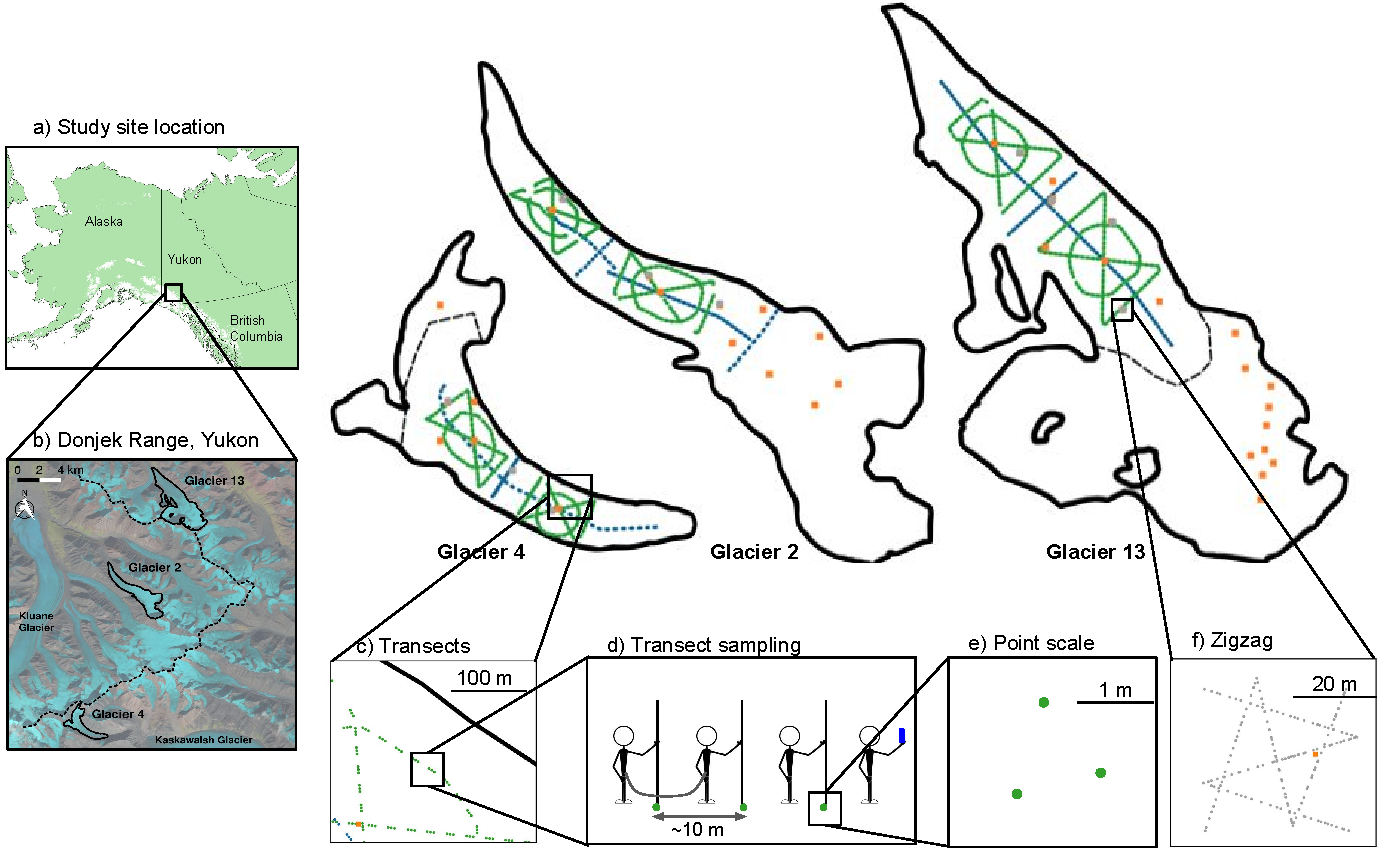
\includegraphics[width =0.9\textwidth]{Sampling.pdf}\\
	\caption{Study area location and sampling design for Glaciers 4, 2 and 13. (a) Study region in the Donjek Range of the St. Elias Mountains of Yukon, Canada. (b) Study glaciers located along a southwest-northeast transect through the Donjek Range. The local topographic divide is shown as a dashed line. Imagery from Landsat8 (5 September 2013, data available from the U.S. Geological Survey). (c) Details of the snow-survey sampling design, with centreline and transverse transects (blue dots), hourglass and circle designs (green dots) and locations of snow density measurements (orange squares). Arrows indicate ice-flow directions. Approximate location of ELA on each glacier is shown as a black dashed line. (d) Close up of linear and curvilinear transects. (e) Configuration of navigator and observers. (f) Point-scale snow-depth sampling. (g) Linear-random snow-depth measurements in `zigzag' design (\DIFdelbeginFL \DIFdelFL{grey }\DIFdelendFL \DIFaddbeginFL \DIFaddFL{red }\DIFaddendFL dots) with one density measurement (orange square) per zigzag.}
	\label{fig:Sampling}
\end{figure*}

\section{Study site}

The St. Elias Mountains (Fig. \ref{fig:Sampling}a) rise sharply from the Pacific Ocean, creating a significant climatic gradient between coastal maritime conditions, generated by Aleutian--Gulf of Alaska low-pressure systems, and interior continental conditions, driven by the Yukon--Mackenzie high-pressure system \citep{Taylor1969}. The boundary between the two climatic zones is generally aligned with the divide between the Hubbard and Kaskawulsh Glaciers, approximately 130\,km from the coast. Research on snow distribution and glacier mass balance in this area is limited. A series of research programs, including Project ``Snow Cornice''  and the Icefield Ranges Research Project, were operational in the 1950s and 60s \citep{Wood1948, Danby2003} and in the last 30 years, there have been a few long-term studies on selected alpine glaciers \citep[e.g.][]{Clarke2014} as well as several regional studies of glacier mass balance and dynamics \citep[e.g.][]{Arendt2008, Burgess2013,Waechter2015}.

We carried out winter balance surveys on three unnamed glaciers in the Donjek Range of the St. Elias Mountains. The Donjek Range is located approximately 40 km to the east of the regional mountain divide and has an area of about $30\times30$\,km$^2$. Glacier 4, Glacier 2 and Glacier 13 (labelling adopted from \cite{Crompton2016}) are located along a southwest-northeast transect through the range (Fig. \ref{fig:Sampling}b, Table \ref{tab:GlacierDetails}). These small alpine glaciers are generally oriented southeast-northwest, with Glacier 4 having a predominantly southeast aspect and Glaciers 2 and 13 have generally northwest aspects. The glaciers are situated in valleys with steep walls and have simple geometries. Based on a detailed study of Glacier 2  \citep{Wilson2013} and related theoretical modelling \citep{Wilson2013a} we suspect all of the study glaciers to be polythermal. 


\begin{table*}[]
\centering
\caption{Physical characteristics of the study glaciers\DIFdelbeginFL \DIFdelFL{and May 2016 winter-balance survey details, including number of snow-depth measurement locations along transects ($n_{\mathrm{T}}$), total length of transects ($d_{\mathrm{T}}$), number of combined snow pit and Federal Sampler density measurement locations ($n_{\rho}$) and number of zigzag surveys ($n_{\mathrm{zz}}$)}\DIFdelendFL .}
\label{tab:GlacierDetails}
\DIFdelbeginFL %DIFDELCMD < \begin{tabular}{cccccccccccc}
%DIFDELCMD < \midrule
%DIFDELCMD < %%%
\DIFdelendFL \DIFaddbeginFL \begin{tabular}{cclccccc}
\hline
\DIFaddendFL \textbf{} & \DIFdelbeginFL \textbf{\DIFdelFL{Location}} %DIFAUXCMD
\DIFdelendFL \DIFaddbeginFL \multicolumn{2}{c}{\textbf{Location}} \DIFaddendFL & \multicolumn{3}{c}{\textbf{Elevation (m a.s.l)}} & \textbf{Slope ($^{\circ}$)} & \DIFdelbeginFL %DIFDELCMD < \multirow{2}{*}{\textbf{\begin{tabular}[c]{@{}c@{}}Area \\ (km$^2$)\end{tabular}}} & \multirow{2}{*}{\textbf{\begin{tabular}[c]{@{}c@{}}Survey\\ Dates\end{tabular}}} & \multicolumn{4}{c}{\textbf{Survey Details}} %%%
\DIFdelendFL \DIFaddbeginFL \multirow{2}{*}{\textbf{\begin{tabular}[c]{@{}c@{}}Area\\ (km$^2$)\end{tabular}}} \DIFaddendFL \\
 & \DIFdelbeginFL \DIFdelFL{UTM Zone 7 }\DIFdelendFL \DIFaddbeginFL \multicolumn{2}{c}{UTM Zone 7} \DIFaddendFL & \textit{Mean} & \textit{Range} & \textit{ELA} & \textit{Mean} &  \DIFdelbeginFL %DIFDELCMD < &  & %%%
\DIFdelFL{$n_{\mathrm{T}}$ }%DIFDELCMD < & %%%
\DIFdelFL{$d_{\mathrm{T}}$ (km) }%DIFDELCMD < & %%%
\DIFdelFL{$n_{\rho}$ }%DIFDELCMD < & %%%
\DIFdelFL{$n_{\mathrm{zz}}$ }\DIFdelendFL \\ \DIFdelbeginFL %DIFDELCMD < \midrule
%DIFDELCMD < %%%
\DIFdelendFL \DIFaddbeginFL \hline
\DIFaddendFL \textbf{Glacier 4} & \DIFdelbeginFL %DIFDELCMD < \begin{tabular}[c]{@{}c@{}}%%%
\DIFdelendFL 595470 E \DIFdelbeginFL %DIFDELCMD < \\ %%%
\DIFdelendFL \DIFaddbeginFL & \DIFaddendFL 6740730 N \DIFdelbeginFL %DIFDELCMD < \end{tabular} %%%
\DIFdelendFL & 2344 & 1958--2809 & $\sim$2500 & 12.8 & 3.8 \DIFdelbeginFL %DIFDELCMD < & %%%
\DIFdelFL{4--7 May 2016 }%DIFDELCMD < & %%%
\DIFdelFL{649 }%DIFDELCMD < & %%%
\DIFdelFL{13.1 }%DIFDELCMD < & %%%
\DIFdelFL{10 }%DIFDELCMD < & %%%
\DIFdelFL{3 }\DIFdelendFL \\
\textbf{Glacier 2} & \DIFdelbeginFL %DIFDELCMD < \begin{tabular}[c]{@{}c@{}}%%%
\DIFdelendFL 601160 E \DIFdelbeginFL %DIFDELCMD < \\ %%%
\DIFdelendFL \DIFaddbeginFL & \DIFaddendFL 6753785 N \DIFdelbeginFL %DIFDELCMD < \end{tabular} %%%
\DIFdelendFL & 2495 & 1899--3103 & $\sim$2500 & 13.0 & 7.0 \DIFdelbeginFL %DIFDELCMD < & %%%
\DIFdelFL{8--11 May 2016 }%DIFDELCMD < & %%%
\DIFdelFL{762 }%DIFDELCMD < & %%%
\DIFdelFL{13.6 }%DIFDELCMD < & %%%
\DIFdelFL{11 }%DIFDELCMD < & %%%
\DIFdelFL{3 }\DIFdelendFL \\
\textbf{Glacier 13} & \DIFdelbeginFL %DIFDELCMD < \begin{tabular}[c]{@{}c@{}}%%%
\DIFdelendFL 604602 E \DIFdelbeginFL %DIFDELCMD < \\ %%%
\DIFdelendFL \DIFaddbeginFL & \DIFaddendFL 6763400 N \DIFdelbeginFL %DIFDELCMD < \end{tabular} %%%
\DIFdelendFL & 2428 & 1923--3067 & $\sim$2380 & 13.4 & 12.6
\DIFaddbeginFL \end{tabular}
\end{table*}


\begin{table*}[]
\centering
\caption{\DIFaddFL{Details of the May 2016 winter-balance survey, including number of snow-depth measurement locations along transects ($n_{\mathrm{T}}$), total length of transects ($d_{\mathrm{T}}$), number of combined snow pit and Federal Sampler density measurement locations ($n_{\rho}$), number of zigzag surveys ($n_{\mathrm{zz}}$), number (as percent of total number of gridcells, and of the number of gridcells in the ablation area) of gridcells sampled ($n_{\mathrm{S}}$) and the elevation range (as percent of total elevations range and of ablation-area elevation range).}}
\label{tab:SurveyDetails}
\begin{tabular}{cccccccc}
\textbf{} \DIFaddendFL & \DIFaddbeginFL \textbf{\DIFaddFL{Date}} & \textbf{\DIFaddFL{$n_{\mathrm{T}}$}} & \textbf{\DIFaddFL{$d_{\mathrm{T}}$ (km)}} & \textbf{\DIFaddFL{$n_{\rho}$}} & \textbf{\DIFaddFL{$n_{\mathrm{zz}}$}} & \textbf{\DIFaddFL{$n_{\mathrm{S}}$}} & \textbf{\DIFaddFL{Elevation range (m\,a.s.l.)}} \\ \hline
\textbf{\DIFaddFL{Glacier 4}} & \DIFaddFL{4--7 May 2016 }& \DIFaddFL{649 }& \DIFaddFL{13.1 }& \DIFaddFL{7 }& \DIFaddFL{3 }& \begin{tabular}[c]{@{}c@{}}\DIFaddFL{295 }\\ \DIFaddFL{(12\%, 21\%)}\end{tabular} & \begin{tabular}[c]{@{}c@{}}\DIFaddFL{2015--2539 }\\ \DIFaddFL{(62\%, 97\%)}\end{tabular} \\
\textbf{\DIFaddFL{Glacier 2}} & \DIFaddFL{8--11 May 2016 }& \DIFaddFL{762 }& \DIFaddFL{13.6 }& \DIFaddFL{7 }& \DIFaddFL{3 }& \begin{tabular}[c]{@{}c@{}}\DIFaddFL{353 }\\ \DIFaddFL{(8\%, 14\%)}\end{tabular} & \begin{tabular}[c]{@{}c@{}}\DIFaddFL{2151--2541 }\\ \DIFaddFL{(32\%, 47\%)}\end{tabular} \\
\textbf{\DIFaddFL{Glacier 13}} & \DIFaddendFL 12--15 May 2016 & 941 & 18.1 & \DIFdelbeginFL \DIFdelFL{20 }\DIFdelendFL \DIFaddbeginFL \DIFaddFL{19 }\DIFaddendFL & 4 \DIFaddbeginFL & \begin{tabular}[c]{@{}c@{}}\DIFaddFL{468 }\\ \DIFaddFL{(6\%, 14\%)}\DIFaddendFL \end{tabular} \DIFaddbeginFL & \begin{tabular}[c]{@{}c@{}}\DIFaddFL{2054--2574 }\\ \DIFaddFL{(45\%,62\%)}\end{tabular}
\end{tabular}
\DIFaddendFL \end{table*}

%%%%%%%%%%%%%%%%%%%%%%%%%%%%%%%%%
%	METHODS
%%%%%%%%%%%%%%%%%%%%%%%%%%%%%%%%%


\section{Methods}

Estimating glacier-wide winter balance \DIFaddbegin \DIFadd{($B_\mathrm{w}$) }\DIFaddend involves transforming measurements of snow depth and density into values of winter balance distributed across a defined grid \DIFaddbegin \DIFadd{($b_\mathrm{w}$)}\DIFaddend . We do this in four steps. (1) Obtain direct measurements of snow depth and density in the field. (2) Assign density values to all depth-measurement locations to calculate point-scale values of \DIFdelbegin \DIFdel{WB }\DIFdelend \DIFaddbegin \DIFadd{$b_\mathrm{w}$ }\DIFaddend at each location. \DIFdelbegin \DIFdel{(}\DIFdelend \DIFaddbegin \DIFadd{Winter balance, measured in units of metres water equivalent (m\,w.e.), can be estimated as the product of snow depth and depth-averaged density. (}\DIFaddend 3) Average all point-scale values \DIFaddbegin \DIFadd{of $b_\mathrm{w}$ }\DIFaddend within each gridcell of a digital elevation model (DEM) to obtain the \DIFdelbegin \DIFdel{gricell-averaged WB}\DIFdelend \DIFaddbegin \DIFadd{gridcell-averaged $b_\mathrm{w}$}\DIFaddend . (4) Interpolate and extrapolate these gridcell-averaged \DIFdelbegin \DIFdel{WB }\DIFdelend \DIFaddbegin \DIFadd{$b_\mathrm{w}$ }\DIFaddend values to obtain estimates of \DIFdelbegin \DIFdel{WB (in m\,w.e.) in }\DIFdelend \DIFaddbegin \DIFadd{$b_\mathrm{w}$ in }\DIFaddend each gridcell across the domain. \DIFaddbegin \DIFadd{$B_\mathrm{w}$ is then calculated by taking the average of all gridcell-averaged $b_\mathrm{w}$ values for each glacier. }\DIFaddend For brevity, we refer to these four steps as (1) field measurements, (2) density assignment, (3) gridcell-averaged \DIFdelbegin \DIFdel{WB }\DIFdelend \DIFaddbegin \DIFadd{$b_\mathrm{w}$ }\DIFaddend and (4) distributed \DIFdelbegin \DIFdel{WB}\DIFdelend \DIFaddbegin \DIFadd{$b_\mathrm{w}$}\DIFaddend . Detailed methodology for each step is outlined below. \DIFaddbegin \DIFadd{We use the SPIRIT SPOT-5 DEM (40$\times$40\,m) from 2005 \mbox{%DIFAUXCMD
\citep{Korona2009} }\hspace{0pt}%DIFAUXCMD
throughout this study. 
}\DIFaddend 

\subsection{Field measurements}

\DIFaddbegin \DIFadd{Our sampling campaign involved four people and occurred between 5--15 May 2016, which falls within the period of historical peak snow accumulation in southwestern Yukon (Yukon Snow Survey Bulletin and Water Supply Forecast, May 1, 2016). Snow depth is generally accepted to be more variable than density \mbox{%DIFAUXCMD
\citep{Elder1991, Clark2011, Lopez2013} }\hspace{0pt}%DIFAUXCMD
so we chose a sampling design that resulted in a high ratio ($\sim$55:1) of snow depth to density measurements. In total, we collected more than 9000 snow-depth measurements and more than 100 density measurements throughout the study area (Table \ref{tab:GlacierDetails}\DIFadd}).
}

\DIFadd{During the field campaign there were two small accumulation events. The first, on 6 May 2016, also involved high winds so accumulation could not be determined. The second, on 10 May 2016, resulted in 0.01\,m\,w.e accumulation measured at one location on Glacier 2. Assuming both accumulation events contributed a uniform 0.01\,m\,w.e accumulation to all study glaciers then our survey did not capture $\sim$3\% and $\sim$2\% of estimated $B_\mathrm{w}$ on Glaciers 4 and 2, respectively. We therefore assume that these accumulation events were negligible and apply no correction. Positive temperatures and clear skies occurred between 11--16 May 2016, which we suspect resulted in melt occurring on Glacier 13. The snow in the lower part of the ablation area of Glacier 13 was isothermal and showed clear signs of melt and metamorphosis. The total amount of melt during the study period was estimated using a degree-day model and found to be small ($\leq$0.01\,m\,w.e., see Supplementary Material) so no corrections were made.
}

\DIFaddend \subsubsection{Sampling design}

The snow surveys were designed to capture variability in snow depth at regional, basin, gridcell and point scales \citep{Clark2011}. To capture variability at the regional scale we chose three glaciers along a transect aligned with the dominant precipitation gradient  (Fig. \ref{fig:Sampling}\DIFaddbegin \DIFadd{b}\DIFaddend ) \citep{Taylor1969}. To account for basin-scale variability, snow depth was measured along linear and curvilinear transects on each glacier (Fig. \ref{fig:Sampling}c) with a sample spacing of 10--60 m (Fig. \ref{fig:Sampling}d). Sample spacing was constrained by protocols for safe glacier travel, while survey scope was constrained by the need to complete all surveys within the period of peak accumulation. We selected centreline and transverse transects as the most commonly used survey designs in winter balance studies \citep[e.g.][]{Kaser2003, Machguth2006} as well as an hourglass pattern with an inscribed circle, which allows for sampling in multiple directions and easy travel (personal communication from C. Parr, 2016). To capture variability at the grid scale, we densely sampled up to four gridcells on each glacier using a linear-random sampling design \DIFaddbegin \DIFadd{\mbox{%DIFAUXCMD
\citep{Shea2010} }\hspace{0pt}%DIFAUXCMD
}\DIFaddend we term a `zigzag'. To capture point-scale variability, each observer made 3--4 depth measurements within $\sim$1 m (Fig. \ref{fig:Sampling}\DIFdelbegin \DIFdel{e}\DIFdelend \DIFaddbegin \DIFadd{f}\DIFaddend ) at each transect measurement location. 
\DIFdelbegin \DIFdel{In total, we collected more than 9000 snow-depth measurements throughout the study area (Table \ref{tab:GlacierDetails}). 
}\DIFdelend 

\subsubsection{Snow depth: transects}

\DIFdelbegin \DIFdel{Winter balance can be estimated as the product of snow depth and depth-averaged density. Snow depth is generally accepted to be more variable than density \mbox{%DIFAUXCMD
\citep{Elder1991, Clark2011, Lopez2013} }\hspace{0pt}%DIFAUXCMD
so we chose a sampling design that resulted in a high ratio ($\sim$55:1) of snow depth to density measurements. Our sampling campaign involved four people and occurred between 5--15 May 2016, which falls within the period of historical peak snow accumulation in southwestern Yukon (Yukon Snow Survey Bulletin and Water Supply Forecast, May 1, 2016). }\DIFdelend While roped-up for glacier travel with fixed distances between observers, the lead observer used a single-frequency GPS unit (Garmin GPSMAP 64s) to navigate between predefined transect measurement locations (Fig. \ref{fig:Sampling}e). The remaining three observers used 3.2 m graduated aluminum avalanche probes to make snow-depth measurements \DIFaddbegin \DIFadd{\mbox{%DIFAUXCMD
\citep{Kinar2015}}\hspace{0pt}%DIFAUXCMD
}\DIFaddend . The locations of each set of depth measurements, made by the second, third and fourth observers, are estimated using the recorded location of the first observer, the approximate distance between observers and the direction of travel. \DIFaddbegin \DIFadd{The 3--4 point-scale depth measurements are averaged to obtain a single depth measurement at each transect measurement location. When considering snow variability at the point scale as a source of uncertainty in snow depth measurements, we find that the mean standard deviation of point-scale snow depth measurements is found to be $<$7\% of the mean snow depth for all study glaciers.
}\DIFaddend 

Snow-depth sampling was concentrated in the ablation area to ensure that only snow from the current accumulation season was measured. The boundary between snow and firn in the accumulation area can be difficult to detect and often misinterpreted, especially when using an avalanche probe \citep{Grunewald2010,Sold2013}. We intended to use a firn corer to measure winter balance in the accumulation area, but cold snow combined with positive air temperatures led to cores being unrecoverable. Successful snow depth \DIFdelbegin \DIFdel{and density }\DIFdelend measurements within the accumulation area were made either in snow pits or using a Federal Sampler (described below) to unambiguously identify the snow--firn transition. 

\subsubsection{Snow depth: zigzags}

\DIFdelbegin \DIFdel{To capture snow-depth variability within a single DEM gridcell, we implemented a linear-random zigzag sampling design \mbox{%DIFAUXCMD
\citep{Shea2010}}\hspace{0pt}%DIFAUXCMD
. }\DIFdelend We measured depth at random intervals of 0.3--3.0\,m along two `Z'-shaped patterns \DIFaddbegin \DIFadd{\mbox{%DIFAUXCMD
\citep{Shea2010}}\hspace{0pt}%DIFAUXCMD
}\DIFaddend , resulting in 135--191 measurements per zigzag, within three to four \DIFdelbegin \DIFdel{$40\times40$ }\DIFdelend \DIFaddbegin \DIFadd{40$\times$40\,}\DIFaddend m gridcells (Fig. \ref{fig:Sampling}g) per glacier. Random intervals were machine-generated from a uniform distribution in sufficient numbers that each survey was unique. Zigzag locations were randomly chosen within the upper, middle and lower regions of the ablation area of each glacier. \DIFdelbegin \DIFdel{A fourth zigzag was measured }\DIFdelend \DIFaddbegin \DIFadd{Extra time in the field allowed us to measure a fourth zigzag }\DIFaddend on Glacier 13 in the central ablation area at $\sim$2200 m a.s.l. 

\subsubsection{Snow density}

Snow density was measured using a Snowmetrics wedge cutter in three snow pits on each glacier\DIFdelbegin \DIFdel{, as well as with a Geo Scientific Ltd. metric Federal Sampler. }\DIFdelend \DIFaddbegin \DIFadd{. }\DIFaddend Within the snow pits (SP), we measured a vertical density profile (in \DIFdelbegin \DIFdel{5 }\DIFdelend \DIFaddbegin \DIFadd{10 }\DIFaddend cm increments) with the \DIFdelbegin \DIFdel{$5\times10\times 10$ }\DIFdelend \DIFaddbegin \DIFadd{$5\times5\times 10$ }\DIFaddend cm wedge-shaped cutter (250 cm$^3$) and a Presola 1000\,g spring scale \DIFdelbegin \DIFdel{\mbox{%DIFAUXCMD
\citep[e.g.][]{Gray1981,Fierz2009}}\hspace{0pt}%DIFAUXCMD
}\DIFdelend \DIFaddbegin \DIFadd{\mbox{%DIFAUXCMD
\citep[e.g.][]{Gray1981,Fierz2009,Kinar2015}}\hspace{0pt}%DIFAUXCMD
}\DIFaddend . Wedge-cutter error is approximately $\pm$6\% \citep[e.g.][]{Proksch2016,Carroll1977}. Uncertainty in estimating density from \DIFdelbegin \DIFdel{snow-pit }\DIFdelend \DIFaddbegin \DIFadd{SP }\DIFaddend measurements also stems from incorrect assignment of density to layers that cannot be sampled (e.g. ice lenses and hard layers). We attempt to quantify this uncertainty by varying estimated ice-layer thickness by $\pm$1 cm ($\leq$100\%) of the recorded thickness, ice layer density between 700 and 900\,kg\,m$^{-3}$ and the density of layers identified as being too hard to sample (but not ice) between 600 and 700\,kg\,m$^{-3}$. When considering all three sources of uncertainty, the range of integrated density values is always less than 15\% of the reference density. Depth-averaged densities for shallow pits ($<$50\,cm) that contain ice lenses are particularly sensitive to changes in prescribed density and ice-lens thickness. 

While \DIFdelbegin \DIFdel{snow pits }\DIFdelend \DIFaddbegin \DIFadd{SP }\DIFaddend provide the most accurate measure of snow density, digging and sampling a \DIFdelbegin \DIFdel{snow pit }\DIFdelend \DIFaddbegin \DIFadd{SP }\DIFaddend is time and labour intensive. Therefore, a \DIFdelbegin \DIFdel{Federal Snow }\DIFdelend \DIFaddbegin \DIFadd{Geo Scientific Ltd. metric Federal }\DIFaddend Sampler (FS) \citep{Clyde1932} \DIFaddbegin \DIFadd{with a 3.2--3.8\,cm diameter sampling tube}\DIFaddend , which directly measures depth-integrated snow-water equivalent, was used to augment the \DIFdelbegin \DIFdel{snow pit }\DIFdelend \DIFaddbegin \DIFadd{SP }\DIFaddend measurements. A minimum of three \DIFdelbegin \DIFdel{Federal Sampler }\DIFdelend \DIFaddbegin \DIFadd{FS }\DIFaddend measurements were taken at each of 7--19 locations on each glacier and an additional eight \DIFdelbegin \DIFdel{Federal Sampler }\DIFdelend \DIFaddbegin \DIFadd{FS }\DIFaddend measurements were co-located with \DIFdelbegin \DIFdel{each snow pit profile}\DIFdelend \DIFaddbegin \DIFadd{two SP profiles for each glacier}\DIFaddend . Measurements for which the snow core length inside the sampling tube was less than 90\% of the snow depth were discarded. Densities at each measurement location (eight at each \DIFdelbegin \DIFdel{snow pit}\DIFdelend \DIFaddbegin \DIFadd{SP}\DIFaddend , three elsewhere) were then averaged, with the standard deviation taken to represent the uncertainty. \DIFdelbegin %DIFDELCMD < 

%DIFDELCMD < %%%
\DIFdel{During the field campaign there were two small accumulation events. The first, on 6 May 2016, also involved high winds so accumulation could not be determined. The second, on 10 May 2016, resulted in 0.01 m w.e accumulation measured at one location on Glacier 2. Positive temperatures and clear skies occurred between 11--16 May 2016, which we suspect resulted in melt occurring on Glacier 13. The snow in the lower part of the ablation area of Glacier 13 was isothermal and showed clear signs of melt and metamorphosis. The total amount of accumulation and melt during the study period could not be estimated so no corrections were made}\DIFdelend \DIFaddbegin \DIFadd{The mean standard deviation of FS-derived density was $\leq$4\% of the mean density for all glaciers}\DIFaddend .

\subsection{Density assignment}

Measured snow density must be interpolated or extrapolated to estimate point-scale \DIFdelbegin \DIFdel{winter balance }\DIFdelend \DIFaddbegin \DIFadd{$b_\mathrm{w}$ }\DIFaddend at each snow-depth sampling location. We employ four commonly used methods to interpolate and extrapolate density (Table \ref{tab:densityOptions}): (1) calculate mean density over an entire mountain range \citep[e.g.][]{Cullen2017}, (2) calculate mean density for each glacier \citep[e.g.][]{Elder1991, McGrath2015}, (3) linear regression of density on elevation for each glacier \citep[e.g.][]{Elder1998, Molotch2005} and (4) calculate mean density using inverse-distance weighting \citep[e.g.][]{Molotch2005} for each glacier.  Densities derived from \DIFdelbegin \DIFdel{snow-pit (SP ) measurements and the Federal Sampler (FS ) }\DIFdelend \DIFaddbegin \DIFadd{SP and FS measurements }\DIFaddend are treated separately, for reasons explained below, resulting in eight possible methods of assigning density.

\begin{table}
\centering
\caption{Eight methods used to estimate snow density at unmeasured locations. Total number of resulting density values given in parentheses, with $n_T$ the total number of snow-depth measurement locations along transects (Table \ref{tab:GlacierDetails}).}
\label{tab:densityOptions}
\begin{tabular}{cccc}
\hline
\multirow{2}{*}{\textbf{\begin{tabular}[c]{@{}c@{}}Method \\ code \end{tabular}}} & \multicolumn{2}{c}{\textbf{\begin{tabular}[c]{@{}c@{}}Source of measured \\ snow density\end{tabular}}} & \multirow{2}{*}{\textbf{\begin{tabular}[c]{@{}c@{}}Density assignment \\ method\end{tabular}}} \\
 & \textit{Snow pit} & \textit{\begin{tabular}[c]{@{}c@{}}Federal\\ Sampler\end{tabular}} &  \\ \hline
S1 & $\blacksquare$ &  & \multirow{2}{*}{\begin{tabular}[c]{@{}c@{}}Mean of measurements \\ across all glaciers (1)\end{tabular}} \\
F1 &  & $\blacksquare$ &  \\ \hline
S2 & $\blacksquare$ &  & \multirow{2}{*}{\begin{tabular}[c]{@{}c@{}}Mean of  measurements \\ for each glacier (3)\end{tabular}} \\
F2 &  & $\blacksquare$ &  \\ \hline
S3 & $\blacksquare$ &  & \multirow{2}{*}{\begin{tabular}[c]{@{}c@{}}Regression of density on \\ elevation for a glacier ($n_T$)\end{tabular}} \\
F3 &  & $\blacksquare$ &  \\ \hline
S4 & $\blacksquare$ &  & \multirow{2}{*}{\begin{tabular}[c]{@{}c@{}}Inverse distance weighted\\ mean for a glacier ($n_T$)\end{tabular}} \\
F4 &  & $\blacksquare$ & 
\end{tabular}
\end{table}


\subsection{Gridcell-averaged winter balance}

We average one to six (mean of 2.1 measurements) point-scale values of \DIFdelbegin \DIFdel{WB within each $40 \times 40$\,m }\DIFdelend \DIFaddbegin \DIFadd{$b_\mathrm{w}$ within each }\DIFaddend DEM gridcell to obtain the gricell-averaged \DIFdelbegin \DIFdel{WB}\DIFdelend \DIFaddbegin \DIFadd{$b_\mathrm{w}$}\DIFaddend . The locations of individual measurements have uncertainty due to the error in the horizontal position given by the GPS unit and the estimation of observer location based on the recorded GPS positions of the navigator. This location uncertainty could result in the incorrect assignment of a point-scale \DIFdelbegin \DIFdel{WB }\DIFdelend \DIFaddbegin \DIFadd{$b_\mathrm{w}$ measurement }\DIFaddend to a particular gridcell. However, this source of error is not further investigated because we assume that the uncertainty \DIFdelbegin \DIFdel{in gridcell-averaged WB }\DIFdelend \DIFaddbegin \DIFadd{resulting from incorrect locations of point-scale $b_\mathrm{w}$ values }\DIFaddend is captured in the \DIFdelbegin \DIFdel{zigzag measurements }\DIFdelend \DIFaddbegin \DIFadd{uncertainty derived from zigzag measurements, as }\DIFaddend described below. \DIFdelbegin \DIFdel{Uncertainty }\DIFdelend \DIFaddbegin \DIFadd{Error }\DIFaddend due to having multiple observers \DIFdelbegin \DIFdel{was also evaluated . There are }\DIFdelend \DIFaddbegin \DIFadd{is also evaluated by conducting an analysis of variance (ANOVA) of snow-depth measurement along a transect and testing for differences between observers. We find }\DIFaddend no significant differences between snow-depth measurements made by observers along any transect (p$>$0.05), with the exception of the first transect on Glacier 4 (51 measurements)\DIFdelbegin \DIFdel{. 
}\DIFdelend \DIFaddbegin \DIFadd{, where snow depth values collected by one observer were, on average, greater than the snow depth measurements taken by the other two observers (p$<$0.01). Since this was the first transect and the only one to show differences by observer, this difference can be considered an anomaly. We conclude that observer bias is not an important effect in this study and therefore apply no observer corrections to the data.
}\DIFaddend 

\subsection{Distributed winter balance}

Gridcell-averaged values of \DIFdelbegin \DIFdel{WB }\DIFdelend \DIFaddbegin \DIFadd{$b_\mathrm{w}$ }\DIFaddend are interpolated and extrapolated across each glacier using linear regression (LR) and \DIFdelbegin \DIFdel{simple kriging (SK}\DIFdelend \DIFaddbegin \DIFadd{ordinary kriging (OK}\DIFaddend ). The \DIFdelbegin \DIFdel{regression }\DIFdelend \DIFaddbegin \DIFadd{LR }\DIFaddend relates gridcell-averaged \DIFdelbegin \DIFdel{WB and }\DIFdelend \DIFaddbegin \DIFadd{$b_\mathrm{w}$ to }\DIFaddend various topographic parameters \DIFdelbegin \DIFdel{, as this method }\DIFdelend \DIFaddbegin \DIFadd{and we use this method because it }\DIFaddend is simple and has precedent for success \citep[e.g.][]{McGrath2015}. Instead of a basic \DIFdelbegin \DIFdel{regression }\DIFdelend \DIFaddbegin \DIFadd{LR }\DIFaddend however, we use cross-validation \DIFdelbegin \DIFdel{and }\DIFdelend \DIFaddbegin \DIFadd{to prevent data overfitting as well as }\DIFaddend model averaging to \DIFdelbegin \DIFdel{test }\DIFdelend \DIFaddbegin \DIFadd{allow for }\DIFaddend all combinations of the \DIFaddbegin \DIFadd{chosen }\DIFaddend topographic parameters. We compare the \DIFdelbegin \DIFdel{regression approach with simple kriging (SK)}\DIFdelend \DIFaddbegin \DIFadd{LR approach with OK}\DIFaddend , a data-driven interpolation method free of any physical interpretation \citep[e.g.][]{Hock1999}.

\subsubsection{Linear regression}

In the \DIFdelbegin \DIFdel{regression}\DIFdelend \DIFaddbegin \DIFadd{LR}\DIFaddend , we use commonly applied topographic parameters as in \cite{McGrath2015}, including elevation, slope, aspect, curvature, ``northness'' and a wind-redistribution parameter \DIFaddbegin \DIFadd{($Sx$ from \mbox{%DIFAUXCMD
\cite{Winstral2002}}\hspace{0pt}%DIFAUXCMD
)}\DIFaddend ; we add distance-from-centreline as an additional parameter. \DIFaddbegin \DIFadd{Topographic parameters are standardized for use in the LR. For details on data and methods used to estimate the topographic parameters see the Supplementary Material and \mbox{%DIFAUXCMD
\cite{Pulwicki2017}}\hspace{0pt}%DIFAUXCMD
. }\DIFaddend Our sampling design ensured that the ranges of topographic parameters associated with our measurement locations represent more than 70\% of the total area of each glacier (except elevation on Glacier 2, where our measurements captured only 50\%). 
\DIFdelbegin \DIFdel{Topographic parameters are standardized and then weighted by }\DIFdelend \DIFaddbegin 

\DIFadd{The goal of the LR is to obtain }\DIFaddend a set of fitted regression coefficients ($\beta_i$) \DIFdelbegin \DIFdel{calculated by minimizing the sum of squares of the vertical deviations of each datum from the regression line \mbox{%DIFAUXCMD
\citep{Davis1986}}\hspace{0pt}%DIFAUXCMD
. For details on data and methods used to estimate the topographic parameters see the Supplementary Material. }%DIFDELCMD < 

%DIFDELCMD < %%%
\DIFdel{To }\DIFdelend \DIFaddbegin \DIFadd{that correspond to each topographic parameter and to a model intercept. The LR implemented in this study is an extension of a basic multiple linear regression; we use cross-validation to }\DIFaddend avoid overfitting the data and \DIFaddbegin \DIFadd{model averaging }\DIFaddend to incorporate every possible combination of topographic parameters\DIFdelbegin \DIFdel{, cross-validation and model averaging are implemented. 
}\DIFdelend \DIFaddbegin \DIFadd{. 
}

\DIFaddend First, cross-validation is used to obtain a set of $\beta_i$ \DIFdelbegin \DIFdel{values }\DIFdelend that have the greatest predictive ability \DIFaddbegin \DIFadd{\mbox{%DIFAUXCMD
\citep{Kohavi1995}}\hspace{0pt}%DIFAUXCMD
}\DIFaddend . We randomly select 1000 subsets of the data (2/3 of the values) \DIFdelbegin \DIFdel{to fit the LR and }\DIFdelend \DIFaddbegin \DIFadd{and fit a basic multiple linear regression (implemented in MATLAB) to the data subsets, thus obtaining 1000 sets of $\beta_i$. The basic multiple linear regression calculates a set of $\beta_i$ by minimizing the sum of squares of the vertical deviations of each datum from the regression line \mbox{%DIFAUXCMD
\citep{Davis1986}}\hspace{0pt}%DIFAUXCMD
. Distributed $b_\mathrm{w}$ is then calculated using each set of $\beta_i$ by weighting topographic parameters by their corresponding $\beta_i$ values for all DEM gridcells. We then }\DIFaddend use the remaining data (1/3 of the values) to calculate a root mean squared error (RMSE) \DIFdelbegin \DIFdel{\mbox{%DIFAUXCMD
\citep{Kohavi1995}}\hspace{0pt}%DIFAUXCMD
}\DIFdelend \DIFaddbegin \DIFadd{between the estimated $b_\mathrm{w}$ and the observed $b_\mathrm{w}$ for corresponding locations}\DIFaddend . From the 1000 sets of $\beta_i$ values, we select the set that results in the lowest RMSE. 
\DIFaddbegin 

\DIFaddend Second, we use model averaging to account for uncertainty when selecting predictors and to maximize the model's predictive ability \citep{Madigan1994}. Models are generated by calculating a set of $\beta_i$ \DIFaddbegin \DIFadd{(}\DIFaddend as described above\DIFaddbegin \DIFadd{) }\DIFaddend for all possible combinations of topographic parameters\DIFdelbegin \DIFdel{(}\DIFdelend \DIFaddbegin \DIFadd{, resulting in }\DIFaddend 2$^7$ models \DIFaddbegin \DIFadd{(i.e. 2$^7$ sets of $\beta_i$ with the greatest predictive ability for each linear combination of topographic parameters}\DIFaddend ). Using a Bayesian framework, model averaging involves weighting all models by their posterior model probabilities \citep{Raftery1997}. \DIFdelbegin \DIFdel{To obtain the final regression coefficients, the $\beta_i$ values from each model are weighted according to the }\DIFdelend \DIFaddbegin \DIFadd{We weight the models according to their }\DIFaddend relative predictive success\DIFdelbegin \DIFdel{of the model}\DIFdelend , as assessed by the value of the Bayesian Information Criterion (BIC) \citep{Burnham2004}. BIC penalizes more complex models\DIFaddbegin \DIFadd{, }\DIFaddend which further reduces the risk of overfitting. The \DIFdelbegin \DIFdel{distributed WB is then }\DIFdelend \DIFaddbegin \DIFadd{final set of $\beta_i$ is then the weighted sum of $\beta_i$ from all models. Distributed $b_\mathrm{w}$ is }\DIFaddend obtained by applying the \DIFdelbegin \DIFdel{resulting regression coefficients }\DIFdelend \DIFaddbegin \DIFadd{final set of $\beta_i$ }\DIFaddend to the topographic parameters associated with each gridcell. 

\subsubsection{\DIFdelbegin \DIFdel{Simple }\DIFdelend \DIFaddbegin \DIFadd{Ordinary }\DIFaddend kriging}

\DIFdelbegin \DIFdel{Simple kriging (SK) }\DIFdelend \DIFaddbegin \DIFadd{Kriging }\DIFaddend is a data-driven method of estimating variables at unsampled locations by using the isotropic spatial correlation (covariance) of measured values to find a set of optimal weights \citep{Davis1986, Li2008}. \DIFdelbegin \DIFdel{Simple kriging }\DIFdelend \DIFaddbegin \DIFadd{Kriging }\DIFaddend assumes spatial correlation between sampling locations that are distributed across a surface and then applies the correlation to interpolate between these locations. \DIFaddbegin \DIFadd{Many forms of kriging have been developed to accommodate different data types \mbox{%DIFAUXCMD
\citep[e.g.][and sources within]{Li2008}}\hspace{0pt}%DIFAUXCMD
. Ordinary kriging (OK) is the most basic form of kriging where the mean of the estimated field is unknown. Unlike LR, OK is not useful for generating hypotheses to explain the physical controls on snow distribution, nor can it be used to estimate winter balance on unmeasured glaciers. However, we chose to use OK because it does not require external inputs and is therefore a means of obtaining $B_\mathrm{w}$ that is free of physical interpretation beyond the information contained in the covariance matrix.
}

\DIFaddend We used the \texttt{DiceKriging} R package \citep{Roustant2012} to calculate the maximum likelihood covariance matrix, as well as the range distance ($\theta$) and nugget for gridcell-averaged values of winter balance. The range distance is a measure of data correlation length and the nugget is the residual that encompasses sampling-error variance as well as the spatial variance at distances less than the minimum sample spacing \citep{Li2008}. \DIFdelbegin \DIFdel{Unlike topographic regression, simple kriging is not useful for generating hypotheses to explain the physical controls on snow distribution, nor can it be used to estimate winter balance on unmeasured glaciers}\DIFdelend \DIFaddbegin \DIFadd{A Mat\'ere covariance function with $\nu$=5/2 is used to define a stationary and isotropic covariance and covariance kernels are parameterized as in \mbox{%DIFAUXCMD
\cite{Rasmussen2006}}\hspace{0pt}%DIFAUXCMD
}\DIFaddend . 

\subsection{Uncertainty analysis \DIFaddbegin \DIFadd{using a Monte Carlo approach}\DIFaddend }

\DIFaddbegin \DIFadd{Three sources of uncertainty are considered separately: the uncertainty due to (1) grid-scale variability of $b_\mathrm{w}$ ($\sigma_{\mathrm{GS}}$), (2) the assignment of snow density ($\sigma_{\rho}$) and (3) interpolating and extrapolating gridcell-averaged values of $b_\mathrm{w}$ ($\sigma_{\mathrm{INT}}$). }\DIFaddend To quantify the uncertainty \DIFaddbegin \DIFadd{of grid-scale and interpolation uncertainty }\DIFaddend on estimates of \DIFdelbegin \DIFdel{glacier-wide WB }\DIFdelend \DIFaddbegin \DIFadd{$B_\mathrm{w}$ }\DIFaddend we conduct a Monte Carlo analysis, which uses repeated random sampling of input variables to calculate a distribution of output variables \citep{Metropolis1949}. We repeat the random sampling process 1000 times, resulting in a distribution of values of the \DIFdelbegin \DIFdel{glacier-wide WB }\DIFdelend \DIFaddbegin \DIFadd{$B_\mathrm{w}$ }\DIFaddend based on uncertainties associated with the four steps outlined above. 
\DIFdelbegin \DIFdel{We use the standard deviation of this distribution as a useful metric of uncertainty on the glacier-wide WB. Three }\DIFdelend \DIFaddbegin \DIFadd{Individual }\DIFaddend sources of uncertainty are \DIFdelbegin \DIFdel{considered separately: the uncertainty due to (1) grid-scale variability of WB ($\sigma_{\mathrm{GS}}$), (2) the assignment of snow density ($\sigma_{\rho}$) and (3) interpolating and extrapolating gridcell-averaged values of WB ($\sigma_{\mathrm{INT}}$). These individual sources of uncertainty are }\DIFdelend propagated through the conversion of snow depth and density measurements to \DIFdelbegin \DIFdel{glacier-wide WB}\DIFdelend \DIFaddbegin \DIFadd{$B_\mathrm{w}$}\DIFaddend . Finally, the combined effect of all three sources of uncertainty on the \DIFdelbegin \DIFdel{glacier-wide WB }\DIFdelend \DIFaddbegin \DIFadd{$B_\mathrm{w}$ }\DIFaddend is quantified. We \DIFaddbegin \DIFadd{use the standard deviation of the distribution of $B_\mathrm{w}$ as a useful metric of $B_\mathrm{w}$ uncertainty. Density assignment uncertainty is calculated as the standard deviation of the eight resulting values of $B_\mathrm{w}$. We }\DIFaddend calculate a relative uncertainty\DIFaddbegin \DIFadd{, }\DIFaddend as the normalized sum of differences between every pair of one hundred distributed \DIFdelbegin \DIFdel{WB }\DIFdelend \DIFaddbegin \DIFadd{$b_\mathrm{w}$ }\DIFaddend estimates including $\sigma_{\mathrm{GS}}$ and $\sigma_{\mathrm{INT}}$\DIFaddbegin \DIFadd{, to investigate the spatial patterns in $b_\mathrm{w}$ uncertainty}\DIFaddend .

	\subsubsection{Grid-scale uncertainty ($\sigma_{\mathrm{GS}}$)}
We make use of the zigzag surveys to quantify the true variability of \DIFdelbegin \DIFdel{WB }\DIFdelend \DIFaddbegin \DIFadd{$b_\mathrm{w}$ }\DIFaddend at the grid scale. Our limited data do not permit a spatially-resolved assessment of grid-scale uncertainty, so we characterize this uncertainty as uniform across each glacier and represent it by a normal distribution. The distribution is centred at zero and has a standard deviation equal to the mean standard deviation of all zigzag measurements for each glacier. For each iteration of the Monte Carlo, \DIFdelbegin \DIFdel{WB }\DIFdelend \DIFaddbegin \DIFadd{$b_\mathrm{w}$ }\DIFaddend values are randomly chosen from the distribution and added to the values of gridcell-averaged \DIFdelbegin \DIFdel{WB}\DIFdelend \DIFaddbegin \DIFadd{$b_\mathrm{w}$}\DIFaddend . These perturbed gridcell-averaged values of \DIFdelbegin \DIFdel{WB }\DIFdelend \DIFaddbegin \DIFadd{$b_\mathrm{w}$ }\DIFaddend are then used in the interpolation. We represent uncertainty in \DIFdelbegin \DIFdel{glacier-wide WB }\DIFdelend \DIFaddbegin \DIFadd{$B_\mathrm{w}$ }\DIFaddend due to grid-scale uncertainty ($\sigma_{\mathrm{GS}}$) as the standard deviation of the resulting distribution of \DIFdelbegin \DIFdel{glacier-wide WB }\DIFdelend \DIFaddbegin \DIFadd{$B_\mathrm{w}$ }\DIFaddend estimates.  

	\subsubsection{Density assignment uncertainty ($\sigma_{\rho}$)}
We incorporate uncertainty due to the method of density assignment by carrying forward all eight density interpolation methods (Table \ref{tab:densityOptions}) when estimating \DIFdelbegin \DIFdel{glacier-wide WB}\DIFdelend \DIFaddbegin \DIFadd{$B_\mathrm{w}$}\DIFaddend . By choosing to retain even the least plausible options, as well as the questionable FS data, this approach results in a generous assessment of uncertainty. We represent the \DIFdelbegin \DIFdel{glacier-wide WB }\DIFdelend \DIFaddbegin \DIFadd{$B_\mathrm{w}$ }\DIFaddend uncertainty due to density assignment uncertainty ($\sigma_{\rho}$) as the standard deviation of \DIFdelbegin \DIFdel{glacier-wide WB }\DIFdelend \DIFaddbegin \DIFadd{$B_\mathrm{w}$ }\DIFaddend estimates calculated using each density assignment method.

	\subsubsection{Interpolation uncertainty ($\sigma_{\mathrm{INT}}$)}
We represent the uncertainty due to interpolation\DIFaddbegin \DIFadd{/extrapolation }\DIFaddend of gridcell-averaged \DIFdelbegin \DIFdel{WB }\DIFdelend \DIFaddbegin \DIFadd{$b_\mathrm{w}$ }\DIFaddend in different ways for LR and \DIFdelbegin \DIFdel{SK}\DIFdelend \DIFaddbegin \DIFadd{OK}\DIFaddend . LR interpolation uncertainty is represented by a multivariate normal distribution of possible regression coefficients ($\beta_i$). The standard deviation of each distribution is calculated using the covariance of \DIFdelbegin \DIFdel{regression coefficients }\DIFdelend \DIFaddbegin \DIFadd{$\beta_i$ }\DIFaddend as outlined in \cite{Bagos2015}, which ensures that \DIFdelbegin \DIFdel{regression coefficients }\DIFdelend \DIFaddbegin \DIFadd{$\beta_i$ }\DIFaddend are internally consistent. The $\beta_i$ distributions are randomly sampled and used to calculate gridcell-estimated \DIFdelbegin \DIFdel{WB}\DIFdelend \DIFaddbegin \DIFadd{$b_\mathrm{w}$}\DIFaddend .

\DIFdelbegin \DIFdel{SK }\DIFdelend \DIFaddbegin \DIFadd{OK }\DIFaddend interpolation uncertainty is represented by the \DIFdelbegin \DIFdel{95\% confidence interval for }\DIFdelend \DIFaddbegin \DIFadd{standard deviation for each }\DIFaddend gridcell-estimated \DIFdelbegin \DIFdel{values of WB }\DIFdelend \DIFaddbegin \DIFadd{value of $b_\mathrm{w}$ }\DIFaddend generated by the \texttt{DiceKriging} package. \DIFdelbegin \DIFdel{From this confidence interval, the standard deviation of each gridcell-estimated WB is then calculated. }\DIFdelend The standard deviation of \DIFdelbegin \DIFdel{glacier-wide WB }\DIFdelend \DIFaddbegin \DIFadd{$B_\mathrm{w}$ }\DIFaddend is then found by taking the square root of the average variance of each gridcell-estimated \DIFdelbegin \DIFdel{WB}\DIFdelend \DIFaddbegin \DIFadd{$b_\mathrm{w}$}\DIFaddend . The final distribution of \DIFdelbegin \DIFdel{glacier-wide WB }\DIFdelend \DIFaddbegin \DIFadd{$B_\mathrm{w}$ }\DIFaddend values is centred at the \DIFdelbegin \DIFdel{glacier-wide WB estimated with SK}\DIFdelend \DIFaddbegin \DIFadd{$B_\mathrm{w}$ estimated with OK}\DIFaddend . For simplicity, the standard deviation of \DIFdelbegin \DIFdel{glacier-wide WB }\DIFdelend \DIFaddbegin \DIFadd{$B_\mathrm{w}$ }\DIFaddend values that result from either LR or \DIFdelbegin \DIFdel{SK interpolation}\DIFdelend \DIFaddbegin \DIFadd{OK interpolation/extrapolation }\DIFaddend uncertainty is referred to as $\sigma_{\mathrm{INT}}$.



%%%%%%%%%%%%%%%%%%%%%%%%%%%%%%%%%%%%%%%%%%%
%DIF < %  RESULTS AND DISCUSSION
%DIF > %  RESULTS
%%%%%%%%%%%%%%%%%%%%%%%%%%%%%%%%%%%%%%%%%%%
\section{Results\DIFdelbegin \DIFdel{and Discussion}\DIFdelend }

\subsection{Field measurements}

\begin{figure}
	\centering
	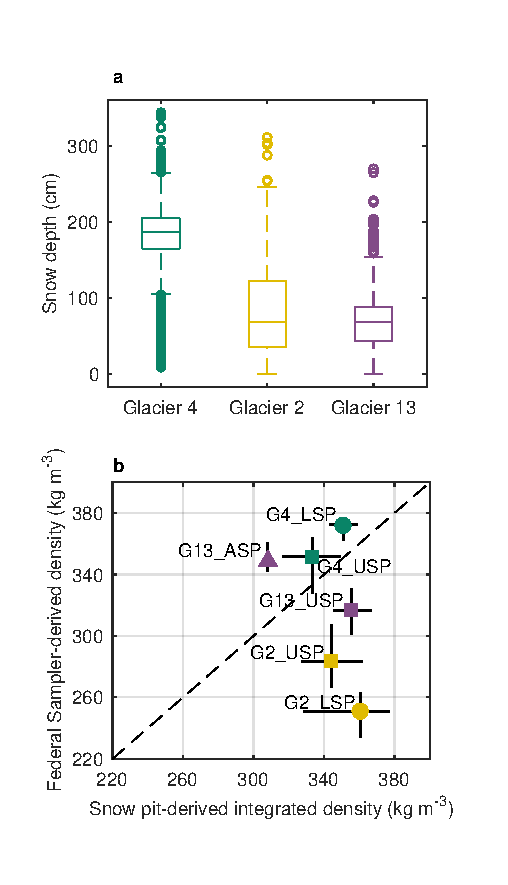
\includegraphics[width =0.35\textwidth]{DepthBoxplot_SPvsFS.pdf}\\
	\caption{Measured snow depth and density. (a) Boxplot of measured snow depth on Glaciers 4, 2 and 13 with the first quartiles (box), median (line within box), minimum and maximum values excluding outliers (bar) and outliers (circles), which are defined as being outside of the range of 1.5 times the quartiles (approximately $\pm2.7\sigma$). (b) Comparison of depth-averaged densities estimated using Federal Sampler (FS) measurements and  a wedge cutter in a snow pit (SP)  for Glacier 4 (G4), Glacier 2 (G2) and Glacier 13 (G13). Labels indicate \DIFdelbeginFL \DIFdelFL{snow pit }\DIFdelendFL \DIFaddbeginFL \DIFaddFL{SP }\DIFaddendFL locations in the accumulation area (ASP), upper ablation area (USP) and lower ablation area (LSP). Error bars for SP-derived densities are calculated by varying the thickness and density of layers that are too hard to sample, and error bars for FS-derived densities are the standard deviation of measurements taken at one location. One-to-one line is dashed.}
	\label{fig:DepthBoxplot_SPvsFS}
\end{figure}

\begin{figure*}
	\centering
	\DIFdelbeginFL %DIFDELCMD < 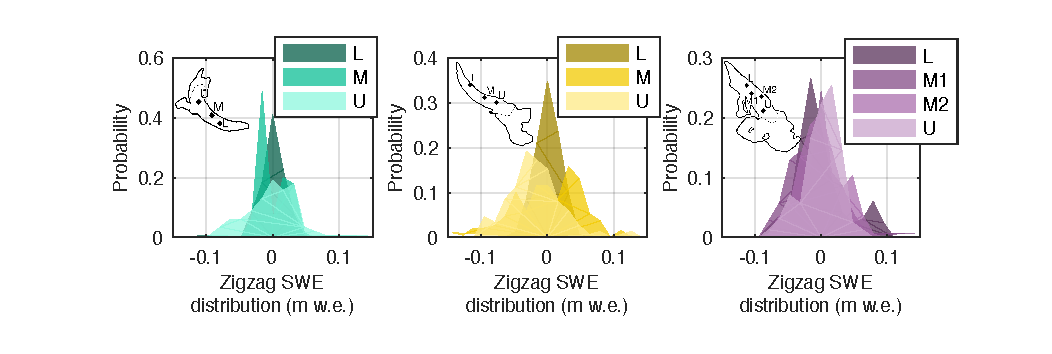
\includegraphics[width =0.8\textwidth]{ZigzagHistogram.pdf}%%%
\DIFdelendFL \DIFaddbeginFL 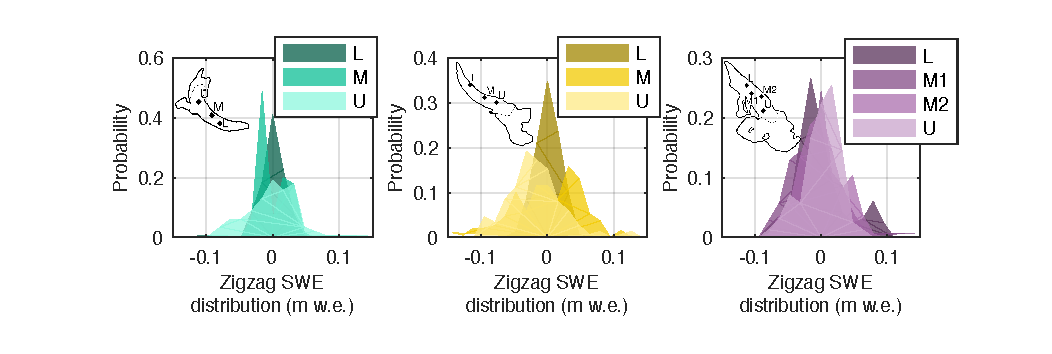
\includegraphics[width =0.7\textwidth]{ZigzagHistogram.pdf}\DIFaddendFL \\
	\caption{Distributions of estimated winter-balance values for each zigzag survey in lower (L), middle (M) and upper (U) ablation areas (insets). Local mean has been subtracted. (a) Glacier 4. (b) Glacier 2. (c) Glacier 13.}
	\label{fig:ZigzagHistogram}
\end{figure*}

\subsubsection{Snow depth}
Mean snow depth varied systematically across the study region, with Glacier 4 having the highest mean snow depth and Glacier 13 having the lowest (Fig. \ref{fig:DepthBoxplot_SPvsFS}\DIFaddbegin \DIFadd{a}\DIFaddend ). At each measurement location, the median range of measured depths (3--4 points) as a percent of the mean local depth is 2\%, 11\% and 12\%, for Glaciers 4, 2 and 13, respectively. While Glacier 4 has the lowest point-scale variability, as assessed above, it also has the highest proportion of outliers, indicating a more variable snow depth across the glacier. The average standard deviation of all zigzag depth measurements is 0.07\,m, 0.17\,m and 0.14\,m, for Glaciers 4, 2 and 13, respectively. When converted to values of \DIFdelbegin \DIFdel{WB }\DIFdelend \DIFaddbegin \DIFadd{$b_\mathrm{w}$ }\DIFaddend using the local FS-derived density measurement, the average standard deviation is 0.027\,m\,w.e., 0.035\,m\,w.e. and 0.040\,m\DIFaddbegin \DIFadd{\,}\DIFaddend w.e. \DIFdelbegin \DIFdel{WB }\DIFdelend \DIFaddbegin \DIFadd{Winter-balance }\DIFaddend data for each zigzag are not normally distributed (Fig. \ref{fig:ZigzagHistogram}).

\subsubsection{Snow density}

Contrary to expectation, co-located FS and SP measurements are found to be uncorrelated (R$^2=0.25$, Fig. \ref{fig:DepthBoxplot_SPvsFS}b). The \DIFdelbegin \DIFdel{Federal Sampler }\DIFdelend \DIFaddbegin \DIFadd{FS }\DIFaddend appears to oversample in deep snow and undersample in shallow snow. Oversampling by small-diameter \DIFdelbegin \DIFdel{(3.2--3.8\,cm) }\DIFdelend sampling tubes has been observed in previous studies, with a percent error between 6.8\% and 11.8\% \citep[e.g.][]{Work1965, Fames1982, Conger2009}. Studies that use \DIFdelbegin \DIFdel{Federal Samplers }\DIFdelend \DIFaddbegin \DIFadd{FS }\DIFaddend often apply a 10\% correction to all measurements for this reason \citep[e.g.][]{Molotch2005}. Oversampling has been attributed to slots ``shaving'' snow into the tube as it is rotated \citep[e.g.][]{Dixon2012} and to snow falling into the slots, particularly for snow samples with densities $>$400\,kg\,m$^{-3}$ and snow depths $>$1\,m \citep[e.g.][]{Beaumont1963}. Undersampling is likely to occur due to loss of snow from the bottom of the sampler \citep{Turcan1975}. Loss by this mechanism may have occurred in our study, given the isothermal and melt-affected snow conditions observed over the lower reaches of Glaciers 2 and 13. Relatively poor \DIFdelbegin \DIFdel{Federal Sampler }\DIFdelend \DIFaddbegin \DIFadd{FS }\DIFaddend spring-scale sensitivity also calls into question the reliability of measurements for snow depths $<$20\,cm.

Our FS-derived density values are positively correlated with snow depth (R$^2= 0.59$). This relationship could be a result of physical processes, such as compaction in deep snow and preferential formation of depth hoar in shallow snow, but is more likely a result of measurement artefacts for a number of reasons. First, the total range of densities measured by the \DIFdelbegin \DIFdel{Federal Sampler }\DIFdelend \DIFaddbegin \DIFadd{FS }\DIFaddend seems improbably large (227--431\,kg\,m$^{-3}$)\DIFdelbegin \DIFdel{given the conditions at the }\DIFdelend \DIFaddbegin \DIFadd{. At the }\DIFaddend time of sampling \DIFaddbegin \DIFadd{the snow pack had little new snow, which confounds the low density values, and was not yet saturated and had few ice lenses, which confounds the high density values}\DIFaddend . Moreover, the range of FS-derived values is much larger than \DIFdelbegin \DIFdel{than }\DIFdelend \DIFaddbegin \DIFadd{that }\DIFaddend of SP-derived values when co-located measurements are compared. Second, compaction effects of the magnitude required to explain the density differences between SP and FS measurements would not be expected at the measured snow depths (up to 340\,cm). Third, no linear relationship exists between depth and SP-derived density (R$^2 = 0.05$). These findings suggest that the \DIFdelbegin \DIFdel{Federal Sampler }\DIFdelend \DIFaddbegin \DIFadd{FS }\DIFaddend measurements have a bias for which we have not identified a suitable correction. \DIFaddbegin \DIFadd{Despite this bias, we use FS-derived densities to generate a range of possible $b_\mathrm{w}$ estimates and to provide a generous estimate of uncertainty arising from density assignment.
}\DIFaddend 

\subsection{Density assignment}

Given the lack of correlation between co-located SP- and FS-derived densities (Fig. \ref{fig:DepthBoxplot_SPvsFS}), we use the densities derived from these two methods separately (Table \ref{tab:densityOptions}). SP-derived regional (S1) and glacier-mean (S2) densities are within one standard deviation of the corresponding FS-derived densities (F1 and F2) although SP-derived density values are larger (see Supplementary Material, Table \DIFdelbegin \DIFdel{S2}\DIFdelend \DIFaddbegin \DIFadd{S3}\DIFaddend ). For both SP- and FS-derived densities, the mean density for any given glacier (S2 or F2) is within one standard deviation of the mean across all glaciers (S1 or F1). Correlations between elevation and SP- and FS-derived densities are generally high (R$^2>$ 0.5) but vary between glaciers (Supplementary material, Table \DIFdelbegin \DIFdel{S2}\DIFdelend \DIFaddbegin \DIFadd{S3}\DIFaddend ). For any given glacier, the standard deviation of the 3--4 SP- or FS-derived densities is $<$13\% of the mean of those values (S2 or F2) (Supplementary material, Table \DIFdelbegin \DIFdel{S2}\DIFdelend \DIFaddbegin \DIFadd{S3}\DIFaddend ). We adopt S2 (glacier-wide mean of SP-derived densities) as the reference method of density assignment. Though the method described by S2 does not account for known basin-scale spatial variability in snow density \citep[e.g.][]{Wetlaufer2016}, it is commonly used in winter balance studies \citep[e.g.][]{Elder1991,McGrath2015,Cullen2017}. 

\subsection{Gridcell-averaged winter balance}

The distributions of gridcell-averaged \DIFdelbegin \DIFdel{WB }\DIFdelend \DIFaddbegin \DIFadd{$b_\mathrm{w}$ }\DIFaddend values for the individual glaciers are similar to those in Fig. \ref{fig:DepthBoxplot_SPvsFS}a but with fewer outliers \DIFdelbegin \DIFdel{. }\DIFdelend \DIFaddbegin \DIFadd{(see Supplementary Material, Fig. S4). }\DIFaddend The standard deviations of \DIFdelbegin \DIFdel{WB }\DIFdelend \DIFaddbegin \DIFadd{$b_\mathrm{w}$ }\DIFaddend values determined from the zigzag surveys are almost twice as large as the mean standard deviation of point-scale \DIFdelbegin \DIFdel{WB }\DIFdelend \DIFaddbegin \DIFadd{$b_\mathrm{w}$ }\DIFaddend values within a gridcell measured along transects \DIFdelbegin \DIFdel{. }\DIFdelend \DIFaddbegin \DIFadd{(see Supplementary Material, Fig. S5). }\DIFaddend However, a small number of gridcells sampled in transect surveys have standard deviations in \DIFdelbegin \DIFdel{WB }\DIFdelend \DIFaddbegin \DIFadd{$b_\mathrm{w}$ }\DIFaddend that exceed 0.25\,m\,w.e. ($\sim$10 times greater than those for zigzag surveys). 
\DIFdelbegin \DIFdel{We nevertheless assume that the gridcell uncertainty is captured with dense sampling in zigzag gridcells. 
}\DIFdelend 

\DIFdelbegin %DIFDELCMD < \begin{figure}
%DIFDELCMD < 	\centering
%DIFDELCMD < 	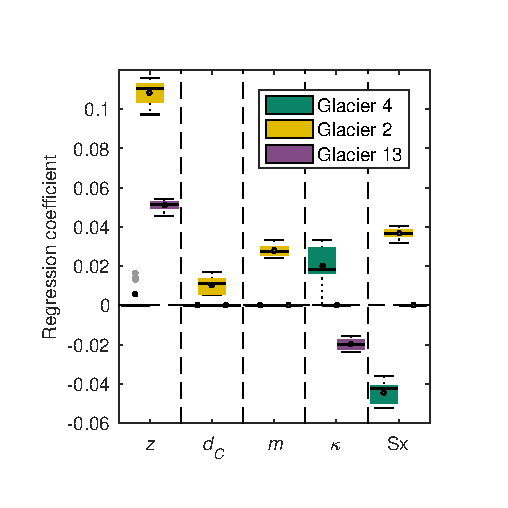
\includegraphics[width =0.4\textwidth]{BetaCoeffs.pdf}\\
%DIFDELCMD < 	\caption{%%%
\DIFdelFL{Distribution of coefficients ($\beta_i$) determined by linear regression of gridcell-averaged WB on DEM-derived topographic parameters for the eight different density assignment methods (Table \ref{tab:densityOptions}). Coefficients are calculated using standardized data, so values can be compared across parameters. Regression coefficients that are not significant are assigned a value of zero. Topographic parameters include elevation ($z$), distance from centreline ($d_C$), slope ($m$), curvature ($\kappa$) and wind redistribution ($Sx$).  Aspect ($\alpha$) and ``northness'' ($N$) are not shown because coefficient values are zero in every case. The box plot shows first quartiles (box), median (line within box), mean (circle within box), minimum and maximum values excluding outliers (bars) and outliers (gray dots), which are defined as being outside of the range of 1.5 times the quartiles (approximately $\pm2.7\sigma$). }%DIFDELCMD < }
%DIFDELCMD < 	%DIFDELCMD < \label{fig:BetaCoeffs}%%%
%DIFDELCMD < \end{figure}
%DIFDELCMD < %%%
\DIFdelend \DIFaddbegin \subsection{\DIFadd{Distributed winter balance}}
\DIFaddend 

\begin{figure}
	\centering
	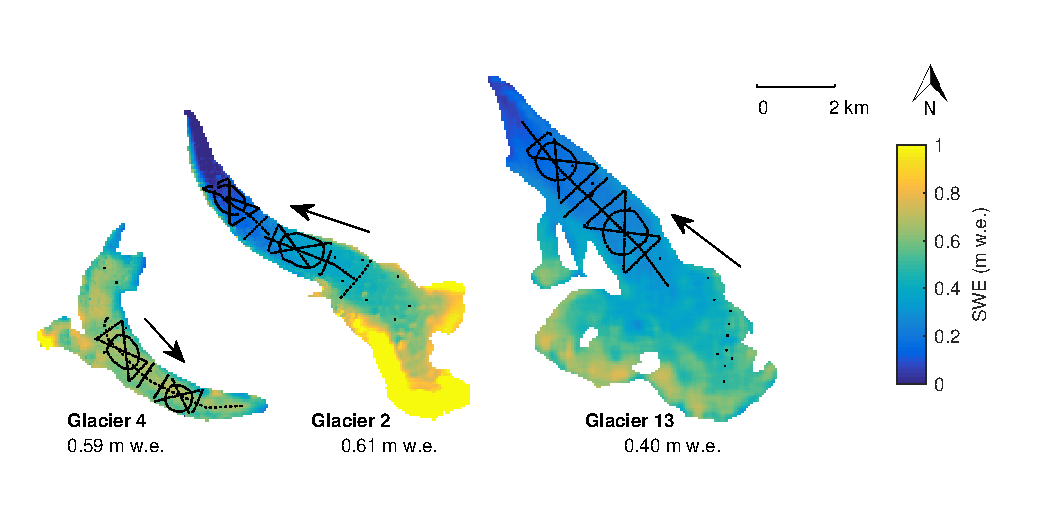
\includegraphics[width =0.5\textwidth]{LR_map.pdf}\\
    \DIFdelbeginFL %DIFDELCMD < 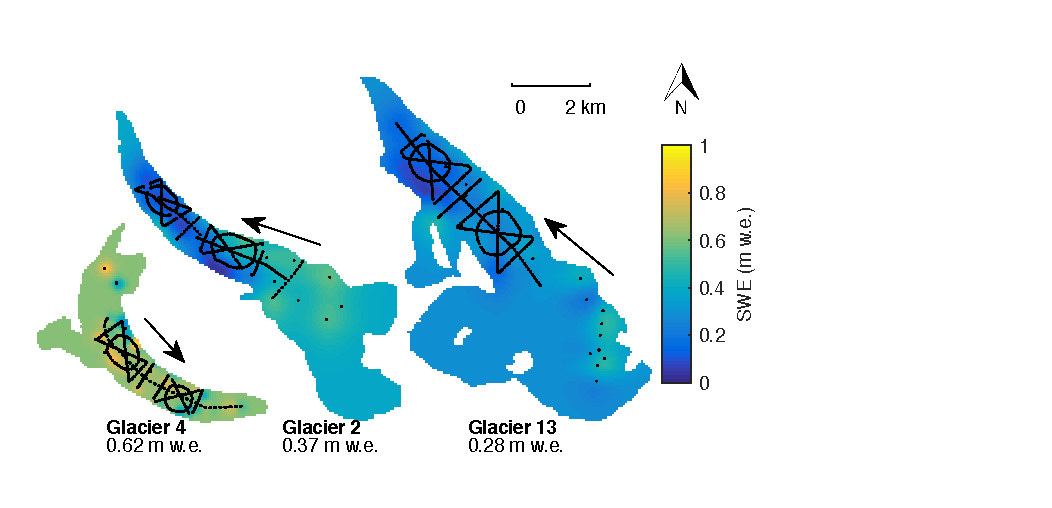
\includegraphics[width =0.5\textwidth]{SK_map.pdf}%%%
\DIFdelendFL \DIFaddbeginFL 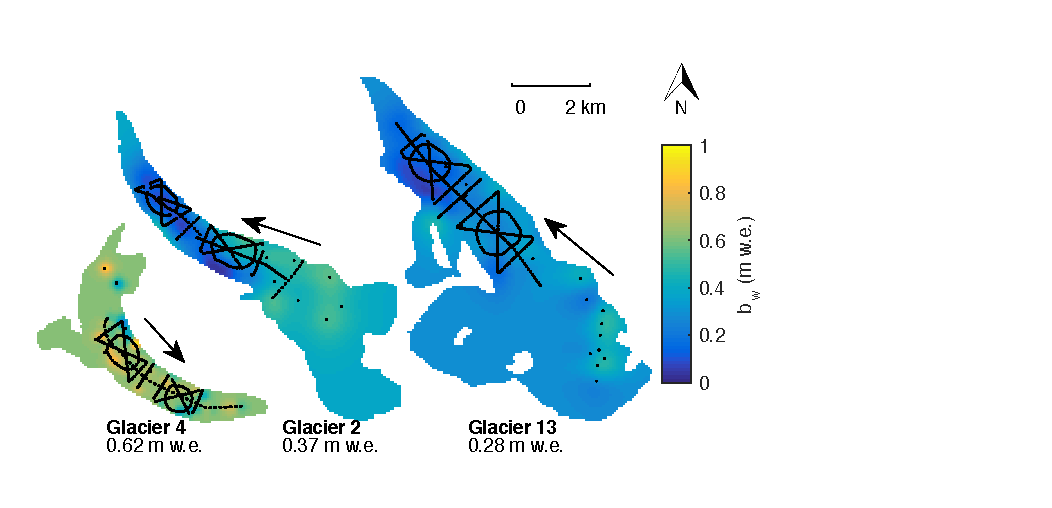
\includegraphics[width =0.5\textwidth]{OK_map.pdf}\DIFaddendFL \\
	\caption{Spatial distribution of winter balance (\DIFdelbeginFL \DIFdelFL{WB}\DIFdelendFL \DIFaddbeginFL \DIFaddFL{$b_\mathrm{w}$}\DIFaddendFL ) estimated using linear regression (top row) and \DIFdelbeginFL \DIFdelFL{simple }\DIFdelendFL \DIFaddbeginFL \DIFaddFL{ordinary }\DIFaddendFL kriging (bottom row) with densities assigned as per S2 (Table \ref{tab:densityOptions}). \DIFaddbeginFL \DIFaddFL{The linear regression (LR) method involves multiplying regression coefficients, found using cross validation and model averaging, by topographic parameters for each gridcell. Ordinary kriging (OK) uses the covariance of measured values to find a set of optimal weights for estimating values at unmeasured locations. }\DIFaddendFL Locations of snow-depth measurements \DIFaddbeginFL \DIFaddFL{made in May 2016 }\DIFaddendFL are shown as black dots. Ice-flow directions are indicated by arrows. Values of \DIFdelbeginFL \DIFdelFL{glacier-wide WB }\DIFdelendFL \DIFaddbeginFL \DIFaddFL{$B_\mathrm{w}$ }\DIFaddendFL are given below labels.}
	\DIFdelbeginFL %DIFDELCMD < \label{fig:LR_OK_map}
%DIFDELCMD < %%%
\DIFdelendFL \DIFaddbeginFL \label{fig:LR_OK_map}
\DIFaddendFL \end{figure}

\DIFdelbegin \subsection{\DIFdel{Distributed winter balance}}
 %DIFAUXCMD
\addtocounter{subsection}{-1}%DIFAUXCMD
\DIFdelend \DIFaddbegin \begin{figure}
	\centering
	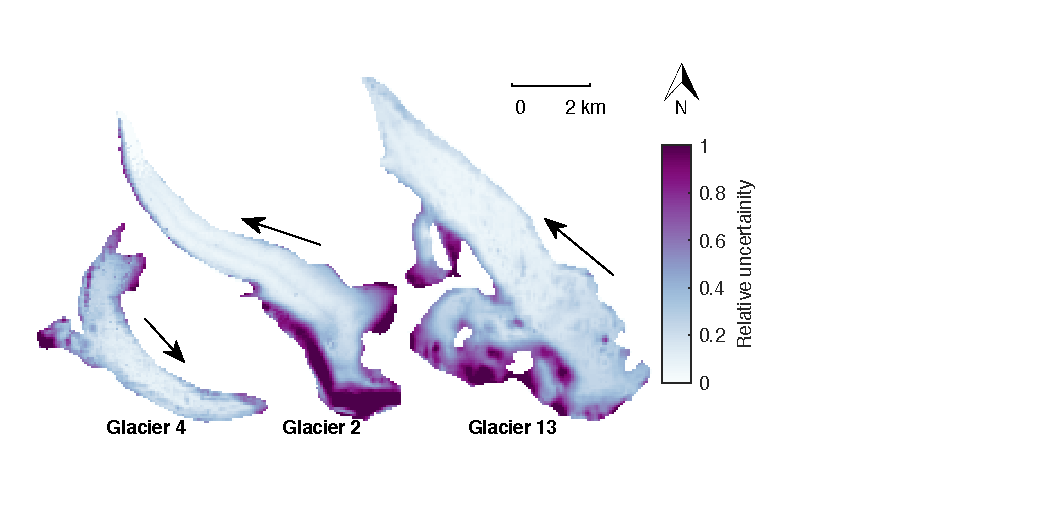
\includegraphics[width =0.5\textwidth]{SpatialVar_LR.pdf}\\
	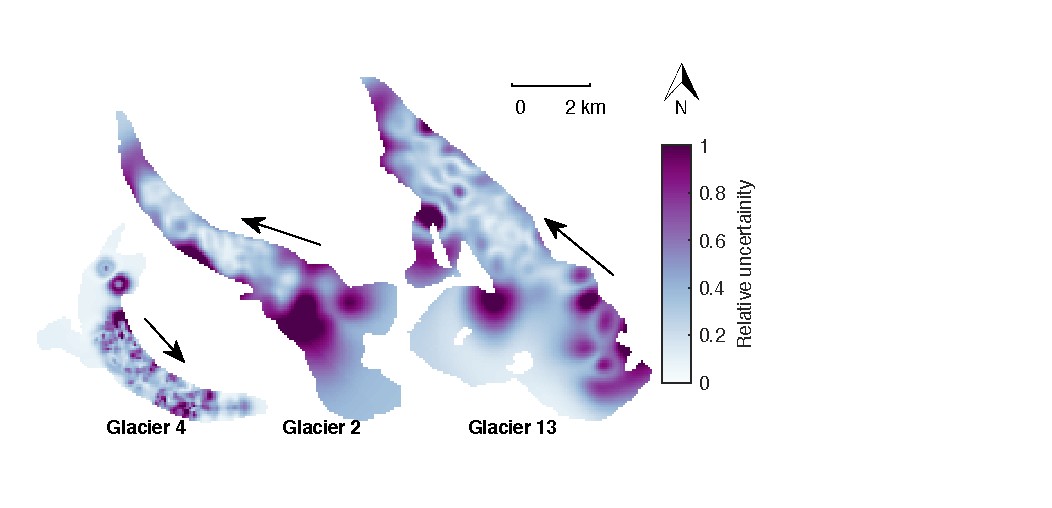
\includegraphics[width =0.5\textwidth]{SpatialVar_OK.pdf}\\
	\caption{\DIFaddFL{Relative uncertainty in distributed winter balance ($b_\mathrm{w}$) (Fig. \ref{fig:LR_OK_map}) found using linear regression (top row) and ordinary kriging (bottom row). Values closer to one indicate higher relative uncertainty. Ice-flow directions are indicated by arrows.}}
	\label{fig:WSMBspatialvar}
\end{figure}
\DIFaddend 

\DIFaddbegin \begin{figure*}
	\centering
	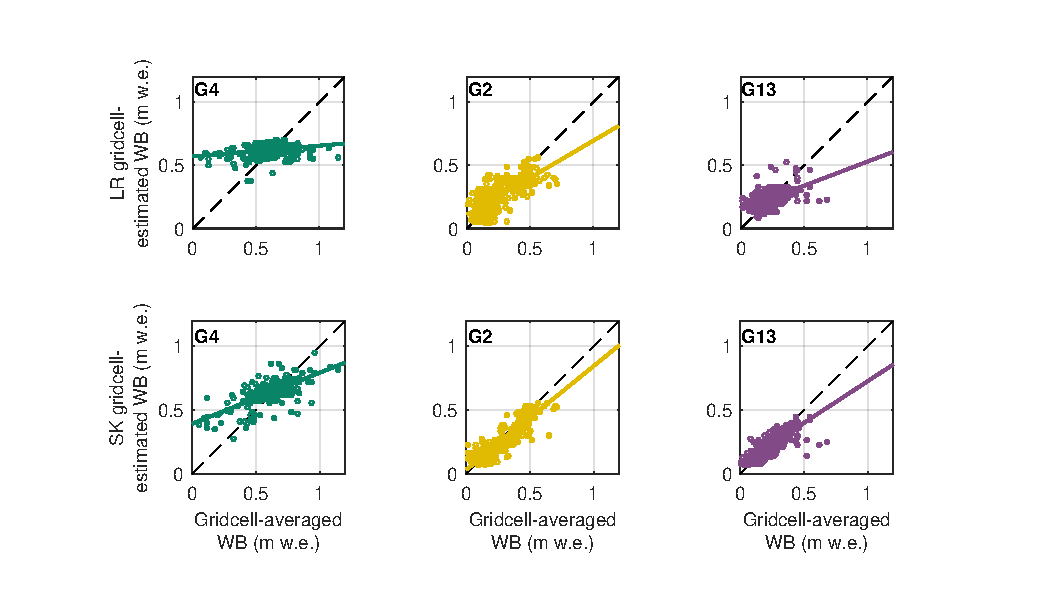
\includegraphics[width =0.7\textwidth]{observedVSestimated_S2.pdf}\\
	\caption{\DIFaddFL{Winter balance ($b_\mathrm{w}$) estimated by linear regression (LR, top row) or ordinary kriging (OK, bottom row) versus the grid-cell averaged $b_\mathrm{w}$ data for Glacier 4 (left), Glacier 2 (middle) and Glacier 13 (right). Each circle represents a single gridcell. Explained variance (R$^2$) is provided. Best-fit (solid) and one-to-one (dashed) lines are shown.}}
	\label{fig:observedVSestimated_S2}
\end{figure*}

\DIFaddend \begin{table}[]
\centering
\caption{Glacier-wide winter balance (\DIFdelbeginFL \DIFdelFL{WB}\DIFdelendFL \DIFaddbeginFL \DIFaddFL{$B_\mathrm{w}$}\DIFaddendFL , m\,w.e.) estimated using linear regression and \DIFdelbeginFL \DIFdelFL{simple }\DIFdelendFL \DIFaddbeginFL \DIFaddFL{ordinary }\DIFaddendFL kriging for the three study glaciers. Root mean squared error (RMSE, m\,w.e.) is computed as the average of all RMSE values between gridcell-averaged values of \DIFdelbeginFL \DIFdelFL{WB }\DIFdelendFL \DIFaddbeginFL \DIFaddFL{$b_\mathrm{w}$ }\DIFaddendFL (the data) that were randomly selected and excluded from interpolation ($1/3$ of all data) and those estimated by interpolation. RMSE as a percent of the \DIFdelbeginFL \DIFdelFL{glacier-wide WB }\DIFdelendFL \DIFaddbeginFL \DIFaddFL{$B_\mathrm{w}$ }\DIFaddendFL is shown in brackets.}
\label{tab:WSMB&RMSE}
\begin{tabular}{c|cc|cc}
 & \multicolumn{2}{c|}{\textbf{Linear regression}} & \DIFdelbeginFL %DIFDELCMD < \multicolumn{2}{c}{\textbf{Simple kriging}} %%%
\DIFdelendFL \DIFaddbeginFL \multicolumn{2}{c}{\textbf{Ordinary kriging}} \DIFaddendFL \\
 & \DIFdelbeginFL \DIFdelFL{WB }\DIFdelendFL \DIFaddbeginFL \DIFaddFL{$B_\mathrm{w}$ }\DIFaddendFL & RMSE & \DIFdelbeginFL \DIFdelFL{WB }\DIFdelendFL \DIFaddbeginFL \DIFaddFL{$B_\mathrm{w}$ }\DIFaddendFL & RMSE \\ \hline
\textbf{G4} & 0.58 & 0.15 (26\%) & 0.62 & \DIFdelbeginFL \DIFdelFL{0.13 (21}\DIFdelendFL \DIFaddbeginFL \DIFaddFL{0.11 \,(18}\DIFaddendFL \%) \\
\textbf{G2} & 0.58 & 0.10 (17\%) & \DIFdelbeginFL \DIFdelFL{0.37 }\DIFdelendFL \DIFaddbeginFL \DIFaddFL{0.35 }\DIFaddendFL & \DIFdelbeginFL \DIFdelFL{0.07 (19}\DIFdelendFL \DIFaddbeginFL \DIFaddFL{0.06 \,(18}\DIFaddendFL \%) \\
\textbf{G13} & 0.38 & 0.08 (21\%) & 0.27 & \DIFdelbeginFL \DIFdelFL{0.07 (26}\DIFdelendFL \DIFaddbeginFL \DIFaddFL{0.06 (21}\DIFaddendFL \%)
\end{tabular}
\end{table}

\DIFdelbegin %DIFDELCMD < \begin{figure}
%DIFDELCMD < 	\centering
%DIFDELCMD < 	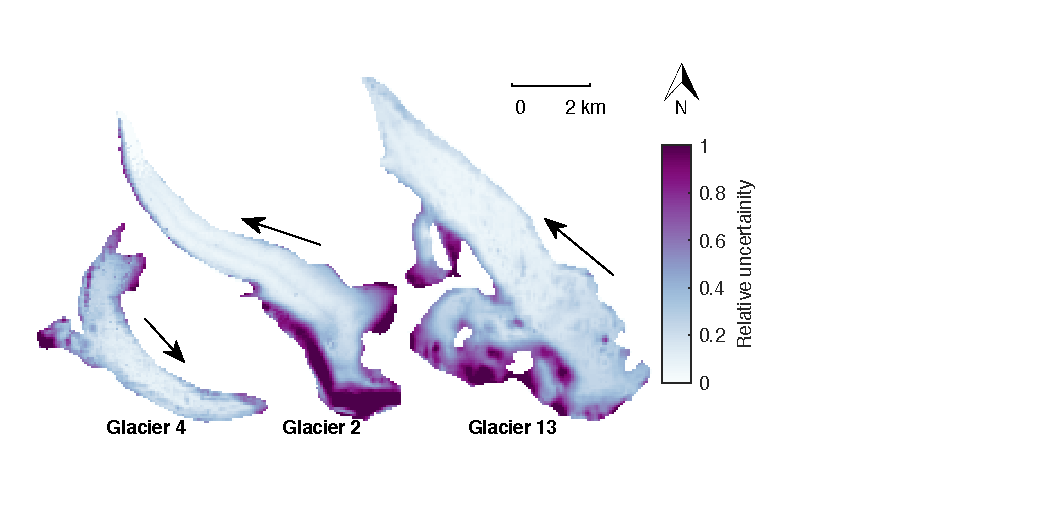
\includegraphics[width =0.5\textwidth]{SpatialVar_LR.pdf}\\
%DIFDELCMD < 	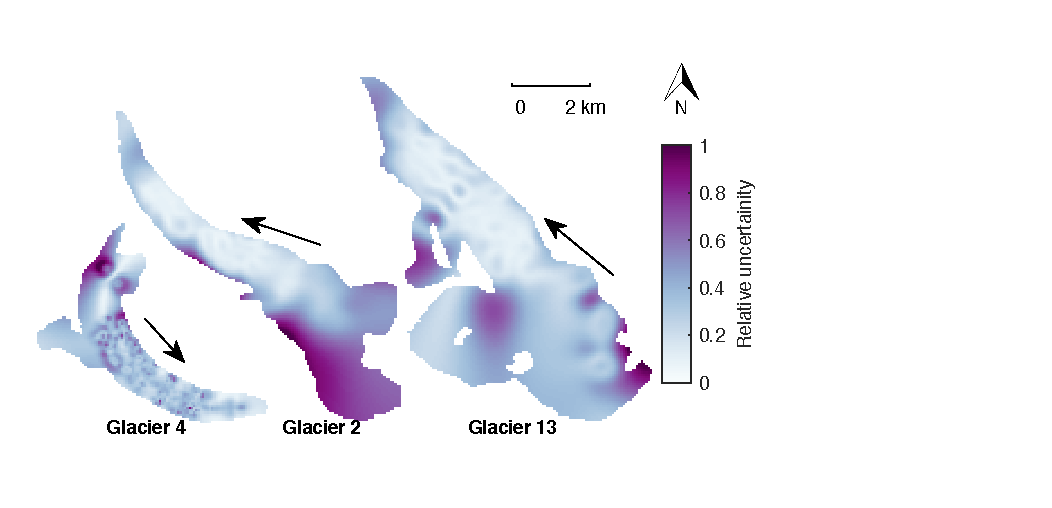
\includegraphics[width =0.5\textwidth]{SpatialVar_SK.pdf}\\
%DIFDELCMD < 	%%%
%DIFDELCMD < \caption{%
{%DIFAUXCMD
\DIFdelFL{Relative uncertainty in distributed winter balance (WB) (Fig. \ref{fig:LR_OK_map}) found using linear regression (top row) and simple kriging (bottom row). Values closer to one indicate higher relative uncertainty. Ice-flow directions are indicated by arrows.}}
	%DIFAUXCMD
%DIFDELCMD < \label{fig:WSMBspatialvar}
%DIFDELCMD < \end{figure}
%DIFDELCMD < %%%
\DIFdelend \DIFaddbegin \subsubsection{\DIFadd{Linear regression}}
\DIFaddend 

\DIFaddbegin \DIFadd{The highest values of estimated $b_\mathrm{w}$ are found in the upper portions of the accumulation areas of Glaciers 2 and 13 (Fig. \ref{fig:LR_OK_map}). These areas also correspond to large values of elevation, slope, and wind redistribution. Extrapolation of the positive relation between $b_\mathrm{w}$ and elevation, as well as slope and $Sx$ for Glacier 2, results in high $b_\mathrm{w}$ estimates and large relative uncertainty in these estimates (Fig. \ref{fig:WSMBspatialvar}). On Glacier 4, the distributed $b_\mathrm{w}$ and the relative uncertainty are almost uniform (Fig. \ref{fig:LR_OK_map}) due to the small regression coefficients for all topographic parameters. The explained variance of the LR-estimated $b_\mathrm{w}$ differs considerably between glaciers (Fig. \ref{fig:observedVSestimated_S2}), with the best correlation between modelled- and observed-$b_\mathrm{w}$ occurring for Glacier 2. LR is an especially poor predictor of $b_\mathrm{w}$ on Glacier 4, where $B_\mathrm{w}$ can be estimated equally well using the mean of the data. RMSE is also highest for Glacier 4 (Table \ref{tab:WSMB&RMSE}). 
}

\subsubsection{\DIFadd{Ordinary kriging}}

\DIFadd{For all three glaciers, large areas that correspond to locations far from measurements have $b_\mathrm{w}$ estimates equal to the kriging mean. Distributed $b_\mathrm{w}$ estimated with OK on Glacier 4 is mostly uniform except for local deviations close to measurement locations (Fig. \ref{fig:LR_OK_map}) and relative uncertainty is highest close to measurement locations.
%DIF >  with $b_\mathrm{w}$ values that differ significantly from the mean at distances approximately equal to the correlation length (Fig. \ref{fig:WSMBspatialvar})??.
Distributed $b_\mathrm{w}$ varies more smoothly on Glaciers 2 and 13 (Fig. \ref{fig:LR_OK_map}). Glacier 2 has a distinct region of low estimated $b_\mathrm{w}$ ($\sim$0.1\,m\,w.e.) in the lower part of the ablation area, which corresponds to a wind-scoured region of the glacier. Glacier 13 has the lowest estimated mean $b_\mathrm{w}$ and only small deviations from this mean at measurement locations (Fig. \ref{fig:LR_OK_map}). Relative uncertainty vary considerably across the three study glaciers  with the greatest uncertainty just outside of the region with observed $b_\mathrm{w}$ (Fig. \ref{fig:WSMBspatialvar}). As expected, explained variance of OK-estimated $b_\mathrm{w}$ is high for both Glaciers 2 and 13 (Fig. \ref{fig:observedVSestimated_S2}) because OK is a data-fitting algorithm. However, explained variance (Fig. \ref{fig:observedVSestimated_S2}) for Glacier 4 is relatively low and RMSE is relatively high (Table \ref{tab:WSMB&RMSE}), indicating a highly variable distribution of $b_\mathrm{w}$.
}

\subsection{\DIFadd{Uncertainty analysis using a Monte Carlo approach}}

\DIFaddend \begin{figure*}
	\centering
	\DIFdelbeginFL %DIFDELCMD < 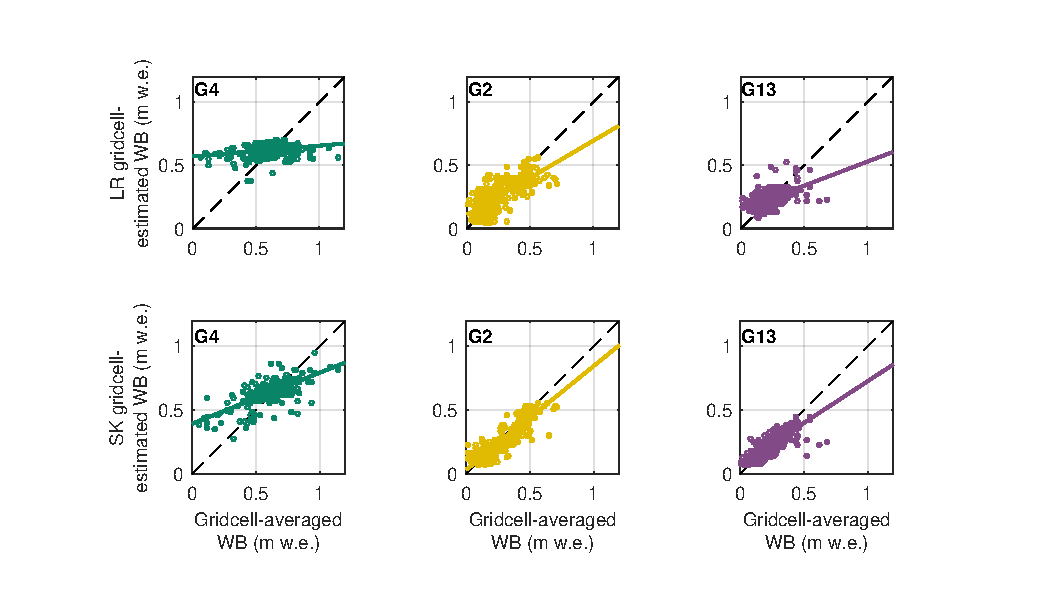
\includegraphics[width =0.7\textwidth]{observedVSestimated_S2.pdf}%%%
\DIFdelendFL \DIFaddbeginFL 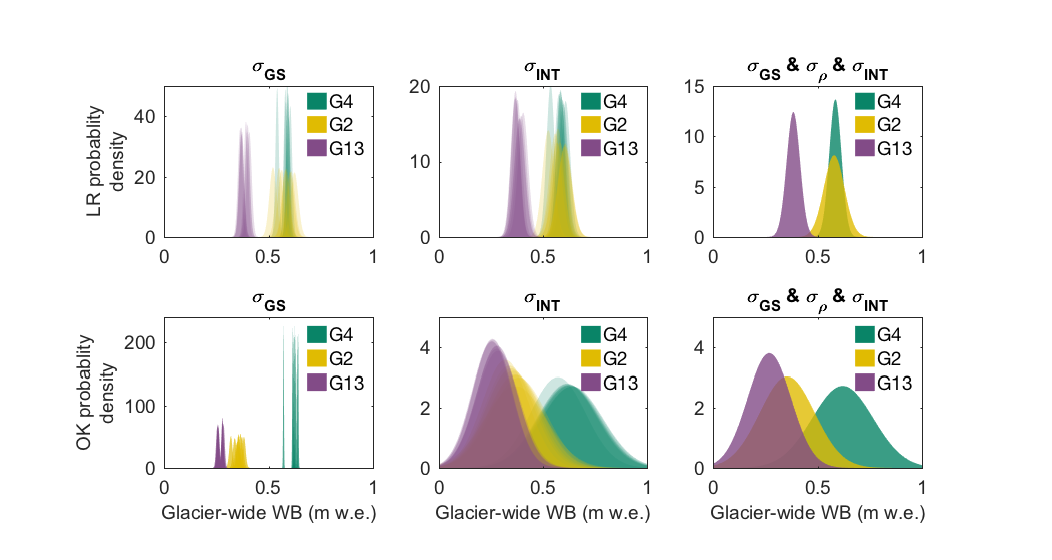
\includegraphics[width =0.95\textwidth]{WSMBDist.pdf}\DIFaddendFL \\
	\caption{\DIFdelbeginFL \DIFdelFL{Winter }\DIFdelendFL \DIFaddbeginFL \DIFaddFL{Distributions of glacier-wide winter }\DIFaddendFL balance (\DIFdelbeginFL \DIFdelFL{WB}\DIFdelendFL \DIFaddbeginFL \DIFaddFL{$B_\mathrm{w}$}\DIFaddendFL ) \DIFdelbeginFL \DIFdelFL{estimated by linear regression }\DIFdelendFL \DIFaddbeginFL \DIFaddFL{for Glaciers 4 }\DIFaddendFL (\DIFdelbeginFL \DIFdelFL{LR}\DIFdelendFL \DIFaddbeginFL \DIFaddFL{G4)}\DIFaddendFL , \DIFdelbeginFL \DIFdelFL{top row}\DIFdelendFL \DIFaddbeginFL \DIFaddFL{2 (G2}\DIFaddendFL ) \DIFdelbeginFL \DIFdelFL{or simple kriging }\DIFdelendFL \DIFaddbeginFL \DIFaddFL{and 13 }\DIFaddendFL (\DIFdelbeginFL \DIFdelFL{SK, bottom row}\DIFdelendFL \DIFaddbeginFL \DIFaddFL{G13}\DIFaddendFL ) \DIFdelbeginFL \DIFdelFL{versus the grid-cell averaged WB data for Glacier 4 }\DIFdelendFL \DIFaddbeginFL \DIFaddFL{that arise from various sources of uncertainty. $B_\mathrm{w}$ distribution arising from grid-scale uncertainty }\DIFaddendFL (\DIFaddbeginFL \DIFaddFL{$\sigma_{\mathrm{GS}}$) (}\DIFaddendFL left \DIFaddbeginFL \DIFaddFL{column}\DIFaddendFL )\DIFdelbeginFL \DIFdelFL{, Glacier 2 }\DIFdelendFL \DIFaddbeginFL \DIFaddFL{. $B_\mathrm{w}$ distribution arising from interpolation uncertainty }\DIFaddendFL (\DIFaddbeginFL \DIFaddFL{$\sigma_{INT}$) (}\DIFaddendFL middle \DIFaddbeginFL \DIFaddFL{column}\DIFaddendFL )\DIFaddbeginFL \DIFaddFL{. $B_\mathrm{w}$ distribution arising from a combination of $\sigma_{\mathrm{GS}}$, $\sigma_{\mathrm{INT}}$ }\DIFaddendFL and \DIFdelbeginFL \DIFdelFL{Glacier 13 }\DIFdelendFL \DIFaddbeginFL \DIFaddFL{density assignment uncertainty }\DIFaddendFL (\DIFaddbeginFL \DIFaddFL{$\sigma_{\rho}$) (}\DIFaddendFL right \DIFaddbeginFL \DIFaddFL{column}\DIFaddendFL ). \DIFdelbeginFL \DIFdelFL{Each circle represents a single gridcell}\DIFdelendFL \DIFaddbeginFL \DIFaddFL{Results are shown for interpolation by linear regression (LR, top row) and ordinary kriging (OK, bottom row)}\DIFaddendFL . \DIFdelbeginFL \DIFdelFL{Best-fit }\DIFdelendFL \DIFaddbeginFL \DIFaddFL{Left two columns include eight distributions per glacier }\DIFaddendFL (\DIFdelbeginFL \DIFdelFL{solid}\DIFdelendFL \DIFaddbeginFL \DIFaddFL{colour}\DIFaddendFL ) and \DIFdelbeginFL \DIFdelFL{one-to-one }\DIFdelendFL \DIFaddbeginFL \DIFaddFL{each corresponds to a density assignment method }\DIFaddendFL (\DIFdelbeginFL \DIFdelFL{dashed}\DIFdelendFL \DIFaddbeginFL \DIFaddFL{S1--S4 and F1--F4}\DIFaddendFL )\DIFdelbeginFL \DIFdelFL{lines are shown}\DIFdelendFL .}
	\DIFdelbeginFL %DIFDELCMD < \label{fig:observedVSestimated_S2}
%DIFDELCMD < %%%
\DIFdelendFL \DIFaddbeginFL \label{fig:WSMBDist_LR}
\DIFaddendFL \end{figure*}

\DIFdelbegin \subsubsection{\DIFdel{Linear Regression}}
%DIFAUXCMD
\addtocounter{subsubsection}{-1}%DIFAUXCMD
\DIFdelend \DIFaddbegin \begin{table*}[]
\centering
\caption{\DIFaddFL{Standard deviation ($\times10^{-2}$\,m\,w.e.) of glacier-wide winter balance ($B_\mathrm{w}$) distributions arising from uncertainties in grid-scale $b_\mathrm{w}$ ($\sigma_{\mathrm{GS}}$), density assignment ($\sigma_{\rho}$), interpolation ($\sigma_{\mathrm{INT}}$) and all three sources combined ($\sigma_{\mathrm{ALL}}$) for linear regression (left columns) and ordinary kriging (right columns)}}
\label{tab:WSMBdistribution_sigma}
\begin{tabular}{c|cccc|cccc}
 & \multicolumn{4}{c|}{\textbf{Linear regression}} & \multicolumn{4}{c}{\textbf{Ordinary kriging}} \\
\textbf{} & \DIFaddFL{$\sigma_{\mathrm{GS}}$ }& \DIFaddFL{$\sigma_{\rho}$ }& \DIFaddFL{$\sigma_{INT}$ }& \DIFaddFL{$\sigma_{ALL}$ }& \DIFaddFL{$\sigma_{\mathrm{GS}}$ }& \DIFaddFL{$\sigma_{\rho}$ }& \DIFaddFL{$\sigma_{INT}$ }& \DIFaddFL{$\sigma_{ALL}$ }\\ \hline
\textbf{\DIFaddFL{Glacier 4}} & \DIFaddFL{0.86 }& \DIFaddFL{1.90 }& \DIFaddFL{2.13 }& \DIFaddFL{2.90 }& \DIFaddFL{0.18 }& \DIFaddFL{2.16 }& \DIFaddFL{14.35 }& \DIFaddFL{14.64 }\\
\textbf{\DIFaddFL{Glacier 2}} & \DIFaddFL{1.80 }& \DIFaddFL{3.37 }& \DIFaddFL{3.09 }& \DIFaddFL{4.90 }& \DIFaddFL{0.80 }& \DIFaddFL{2.06 }& \DIFaddFL{12.65 }& \DIFaddFL{13.14 }\\
\textbf{\DIFaddFL{Glacier 13}} & \DIFaddFL{1.12 }& \DIFaddFL{1.68 }& \DIFaddFL{2.80 }& \DIFaddFL{3.20 }& \DIFaddFL{0.57 }& \DIFaddFL{1.30 }& \DIFaddFL{9.74 }& \DIFaddFL{10.48
}\end{tabular}
\end{table*}
\DIFaddend 

\DIFaddbegin \DIFadd{Glacier-wide winter balance is affected by uncertainty introduced by the representativeness of gridcell-averaged values of $b_\mathrm{w}$ ($\sigma_{\mathrm{GS}}$), choosing a method of density assignment ($\sigma_{\rho}$), and interpolating/extrapolating $b_\mathrm{w}$ values across the domain ($\sigma_{\mathrm{INT}}$). Using a Monte Carlo analysis, we find that interpolation uncertainty contributes more to $B_\mathrm{w}$ uncertainty than grid-scale uncertainty or density assignment method. In other words, the distribution of $B_\mathrm{w}$ that arises from grid-scale uncertainty and the differences in distributions between methods of density assignment are smaller than the distribution that arises from interpolation uncertainty (Fig. \ref{fig:WSMBDist_LR} and Table \ref{tab:WSMBdistribution_sigma}). The $B_\mathrm{w}$ distributions obtained using LR and OK overlap for a given glacier, but the distribution modes differ (Fig. \ref{fig:WSMBDist_LR}). OK-estimated values of $b_\mathrm{w}$ in the accumulation area are generally lower (Fig. \ref{fig:LR_OK_map}), which lowers the $B_\mathrm{w}$ estimate. The uncertainty in OK-estimated values of $B_\mathrm{w}$ is large, and unrealistic $B_\mathrm{w}$ values of 0\,m\,w.e. can be estimated (Fig. \ref{fig:WSMBDist_LR}).
}

\DIFadd{The values of $B_\mathrm{w}$ for our study glaciers (using LR and S2 density assignment method), with an uncertainty equal to one standard deviation of the distribution found with Monte Carlo analysis, are: 0.59\,$\pm$\,0.03\,m\,w.e. for Glacier 4, 0.61\,$\pm$\,0.05\,m\,w.e. for Glacier 2 and 0.40\,$\pm$\,0.03\,m\,w.e. for Glacier 13. The $B_\mathrm{w}$ uncertainty from the three investigated sources of uncertainty ranges from 0.03\,m w.e (5\%) to 0.05\,m w.e (8\%) for LR estimates and from 0.10\,m w.e (37\%) to 0.15\,m w.e (24\%) for ordinary-kriging estimates (Table \ref{tab:WSMB&RMSE}).
}

%DIF > %%%%%%%%%%%%%%%%%%%%%%%%%%%%%%%%%%%%%%%%%%
%DIF > %  DISCUSSION
%DIF > %%%%%%%%%%%%%%%%%%%%%%%%%%%%%%%%%%%%%%%%%%
\section{\DIFadd{Discussion}}

\subsection{\DIFadd{Distributed winter balance}}

\subsubsection{\DIFadd{Linear regression}}

\begin{figure}
	\centering
	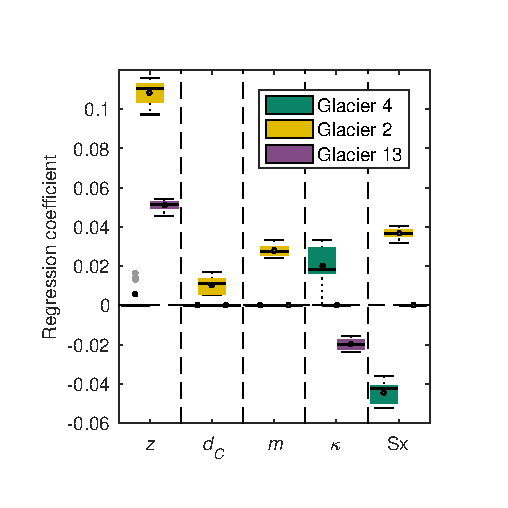
\includegraphics[width =0.4\textwidth]{BetaCoeffs.pdf}\\
	\caption{\DIFaddFL{Distribution of coefficients ($\beta_i$) determined by linear regression of gridcell-averaged $b_\mathrm{w}$ on DEM-derived topographic parameters for the eight different density assignment methods (Table \ref{tab:densityOptions}). Coefficients are calculated using standardized data, so values can be compared across parameters. Regression coefficients that are not significant are assigned a value of zero. Topographic parameters include elevation ($z$), distance from centreline ($d_C$), slope ($m$), curvature ($\kappa$) and wind redistribution ($Sx$).  Aspect ($\alpha$) and ``northness'' ($N$) are not shown because coefficient values are zero in every case. The box plot shows first quartiles (box), median (line within box), mean (circle within box), minimum and maximum values excluding outliers (bars) and outliers (gray dots), which are defined as being outside of the range of 1.5 times the quartiles (approximately $\pm2.7\sigma$). }}
	\label{fig:BetaCoeffs}
\end{figure}

\DIFaddend Of the topographic parameters in the \DIFdelbegin \DIFdel{linear regression}\DIFdelend \DIFaddbegin \DIFadd{LR}\DIFaddend , elevation ($z$) is the most significant predictor of gridcell-averaged \DIFdelbegin \DIFdel{WB }\DIFdelend \DIFaddbegin \DIFadd{$b_\mathrm{w}$ }\DIFaddend for Glaciers 2 and 13, while wind redistribution ($Sx$) is the most significant predictor for Glacier 4 (Fig. \ref{fig:BetaCoeffs}\DIFdelbegin \DIFdel{, Fig. \ref{fig:LR_OK_map}}\DIFdelend ). As expected, gridcell-averaged \DIFdelbegin \DIFdel{WB }\DIFdelend \DIFaddbegin \DIFadd{$b_\mathrm{w}$ }\DIFaddend is positively correlated with elevation where the correlation is significant. It is possible that the elevation correlation was accentuated due to melt onset for Glacier 13 in particular. \DIFdelbegin \DIFdel{Many  studies }\DIFdelend \DIFaddbegin \DIFadd{Glacier 2 had little snow at the terminus likely due to steep slopes and wind-scouring but the snow did not appear to have been affected by melt.  Our results are consistent with many studies that }\DIFaddend have found elevation to be the most significant predictor of \DIFdelbegin \DIFdel{winter-balance data \mbox{%DIFAUXCMD
\citep[e.g.][]{Machguth2006, McGrath2015}}\hspace{0pt}%DIFAUXCMD
. However, WB--elevation gradients vary considerably between glaciers \mbox{%DIFAUXCMD
\citep[e.g.][]{Winther1998} }\hspace{0pt}%DIFAUXCMD
and other factors, such as glacier shape and orientation relative to dominant wind direction, are strong predictors of the winter-balance distribution \mbox{%DIFAUXCMD
\citep{Machguth2006,Grabiec2011}}\hspace{0pt}%DIFAUXCMD
. Some studies find no significant correlation between WB on glaciers and topographic parameters, with }\DIFdelend \DIFaddbegin \DIFadd{seasonal snow accumulation data \mbox{%DIFAUXCMD
\citep[e.g.][]{Machguth2006, Grunewald2014, McGrath2015}}\hspace{0pt}%DIFAUXCMD
. The $b_\mathrm{w}$--elevation gradient is 13\,mm\,100\,m$^{-1}$ on Glacier 2 and 7\,mm\,100\,m$^{-1}$ on Glacier 13. These gradients are consistent with those reported for a few glaciers in Svalbard \mbox{%DIFAUXCMD
\citep{Winther1998} }\hspace{0pt}%DIFAUXCMD
but are considerably smaller than many reported $b_\mathrm{w}$--elevation gradients, which range from about 60 to 240\,mm\,100\,m$^{-1}$ \mbox{%DIFAUXCMD
\citep[e.g.][]{Hagen1990,Tveit1996,Winther1998}}\hspace{0pt}%DIFAUXCMD
. Extrapolating linear relationships to unmeasured locations typically results in considerable estimation error, as seen by the large $b_\mathrm{w}$ values (Fig. \ref{fig:LR_OK_map}) and large relative uncertainty (Fig. \ref{fig:WSMBspatialvar}) in the high-elevation regions of Glaciers 2 and 13. The low correlation between $b_\mathrm{w}$ and elevation on Glacier 4 is consistent with \mbox{%DIFAUXCMD
\cite{Grabiec2011} }\hspace{0pt}%DIFAUXCMD
and \mbox{%DIFAUXCMD
\cite{Lopez2011}}\hspace{0pt}%DIFAUXCMD
, who conclude that }\DIFaddend highly variable distributions of snow \DIFaddbegin \DIFadd{can be }\DIFaddend attributed to complex interactions between topography and the atmosphere that \DIFdelbegin \DIFdel{could not }\DIFdelend \DIFaddbegin \DIFadd{cannot }\DIFaddend be easily quantified\DIFdelbegin \DIFdel{\mbox{%DIFAUXCMD
\citep[e.g.][]{Grabiec2011,Lopez2011}}\hspace{0pt}%DIFAUXCMD
. Extrapolating relationships to unmeasured locations, especially the accumulation area, is susceptible to large uncertainties (Fig. \ref{fig:WSMBspatialvar}). This extrapolation has a considerable effect on values of glacier-wide WB, as the highest values of WB are typically found in the accumulation area  (Fig.
\ref{fig:LR_OK_map}). 
}\DIFdelend \DIFaddbegin \DIFadd{. The snow on Glacier 4 also did not appear to have been affected by melt and it is hypothesized that significant wind-redistribution processes, that were not captured by the $Sx$ parameter, covered ice-topography and produced a relatively uniform snow depth across the glacier.
}\DIFaddend 

Gridcell-averaged \DIFdelbegin \DIFdel{WB }\DIFdelend \DIFaddbegin \DIFadd{$b_\mathrm{w}$ }\DIFaddend is negatively correlated with $Sx$ on Glacier 4, counter-intuitively indicating less snow in what would be interpreted as sheltered areas. Gridcell-averaged \DIFdelbegin \DIFdel{WB }\DIFdelend \DIFaddbegin \DIFadd{$b_\mathrm{w}$ }\DIFaddend is positively correlated with $Sx$ on Glaciers 2 and 13. \DIFdelbegin \DIFdel{Similarly, gridcell-averaged WB is positively correlated with curvature on Glacier 4 and negatively correlated on Glaciers 2 and 13. Wind redistribution and preferential deposition of snow are known to have a large influence on snow distribution at sub-basin scales \mbox{%DIFAUXCMD
\citep[e.g.][]{Dadic2010, Winstral2013,Gerber2017}}\hspace{0pt}%DIFAUXCMD
. Our }\DIFdelend \DIFaddbegin \DIFadd{Our results corroborate those of \mbox{%DIFAUXCMD
\cite{McGrath2015} }\hspace{0pt}%DIFAUXCMD
in a study of six glaciers in Alaska (DEM resolutions of 5 m) where elevation and $Sx$ were the only significant parameters for all glaciers; $Sx$ regression coefficients were smaller than elevation regression coefficients, and in some cases, negative. While our }\DIFaddend results point to wind having an impact on snow distribution, \DIFdelbegin \DIFdel{but }\DIFdelend the wind redistribution parameter ($Sx$) may not adequately capture these effects at our study sites. For example, Glacier 4 \DIFdelbegin \DIFdel{is located in a curved valley with steep side }\DIFdelend \DIFaddbegin \DIFadd{has a curvilinear plan-view profile and is surrounded by steep valley }\DIFaddend walls, so specifying a single cardinal direction for wind may not be adequate. Further, the scale of deposition may be smaller than the resolution of the $Sx$ parameter estimated from the DEM. \DIFdelbegin \DIFdel{Our results corroborate those of \mbox{%DIFAUXCMD
\cite{McGrath2015} }\hspace{0pt}%DIFAUXCMD
in a study of six glaciers in Alaska (DEM resolutions of 5 m) where elevation and $Sx$ were the only significant parameters for all glaciers; $Sx$ regression coefficients were smaller than elevation regression coefficients, and in some cases, negative. In addition to wind redistribution, }\DIFdelend \DIFaddbegin \DIFadd{Creation of a parametrization for }\DIFaddend sublimation from blowing snow\DIFdelbegin \DIFdel{has also }\DIFdelend \DIFaddbegin \DIFadd{, which has }\DIFaddend been shown to be an important mechanism of mass loss from ridges \citep[e.g.][]{Musselman2015}\DIFdelbegin \DIFdel{. Incorporating such losses, as well as redistribution and preferential deposition, may be important for improving representations of distributed winter balance}\DIFdelend \DIFaddbegin \DIFadd{, may also increase the explanatory power of LR for our study sites}\DIFaddend .

We find that transfer of LR coefficients between glaciers results in large estimation errors. Regression coefficients from Glacier 4 produce the highest \DIFdelbegin \DIFdel{root mean squared error }\DIFdelend \DIFaddbegin \DIFadd{RMSE }\DIFaddend (0.38\,m\,w.e. on Glacier 2 and 0.40\,m\,w.e. on Glacier 13, see Table \ref{tab:WSMB&RMSE} for comparison) and \DIFdelbegin \DIFdel{glacier-wide WB }\DIFdelend \DIFaddbegin \DIFadd{$B_\mathrm{w}$ }\DIFaddend values are the same for all glaciers (0.64\,m\,w.e.) due to the dominance of the regression intercept. Even if the \DIFdelbegin \DIFdel{regression }\DIFdelend \DIFaddbegin \DIFadd{LR }\DIFaddend is performed with \DIFdelbegin \DIFdel{WB }\DIFdelend \DIFaddbegin \DIFadd{$b_\mathrm{w}$ }\DIFaddend values from all glaciers combined, the resulting coefficients produce large \DIFdelbegin \DIFdel{root mean squared errors }\DIFdelend \DIFaddbegin \DIFadd{RMSE }\DIFaddend when applied to  individual glaciers (0.31\,m\,w.e., 0.15\,m\,w.e. and 0.14\,m\,w.e. for Glaciers 4, 2 and 13, respectively). Our results are consistent with those of \cite{Grunewald2013}, who found that local statistical models cannot be transferred across basins and that regional-scale models are not able to explain the majority of observed variance in winter balance. 

\subsubsection{\DIFdelbegin \DIFdel{Simple }\DIFdelend \DIFaddbegin \DIFadd{Ordinary }\DIFaddend kriging}

\DIFdelbegin \DIFdel{Fitted kriging parameters, including the nugget and spatial correlation length, can provide insight into important scales of winter-balance variability. The model fitted to the gridcell-averaged values of WB for Glacier 4 has a short correlation length (90 m) and large nugget (see Supplementary Material Table S3), suggesting variability in winter balance at smaller scales. Conversely, Glaciers 2 and 13 have longer correlation lengths ($\sim$450\,m) and smaller nuggets, suggesting variability at larger scales. 
Additionally, simple kriging is better able to estimate values of WB for Glaciers 2 and 13 than for Glacier 4 (Fig. \ref{fig:observedVSestimated_S2}). }\DIFdelend Due to a paucity of data, simple kriging produces almost uniform gridcell-estimated \DIFdelbegin \DIFdel{values of winter balance }\DIFdelend \DIFaddbegin \DIFadd{$b_\mathrm{w}$ }\DIFaddend in the accumulation area of each glacier, inconsistent with observations described in the literature \citep[e.g.][]{Machguth2006, Grabiec2011}. \DIFdelbegin \DIFdel{Extrapolation using simple kriging }\DIFdelend \DIFaddbegin \DIFadd{Glacier 4 has the highest estimated mean with large deviations from the mean at measurement locations. The longer correlation lengths of the data for Glaciers 2 and 13 result in a more smoothly varying distributed $b_\mathrm{w}$. As expected, extrapolation using OK }\DIFaddend leads to large uncertainty (Fig. \ref{fig:WSMBspatialvar}), further emphasizing the need for spatially distributed point-scale measurements. 


\subsubsection{LR and \DIFdelbegin \DIFdel{SK }\DIFdelend \DIFaddbegin \DIFadd{OK }\DIFaddend comparison}

\DIFdelbegin \DIFdel{Glacier-wide WB estimates found using both LR and SK are }\DIFdelend \DIFaddbegin \DIFadd{LR and OK produce similar estimates of distributed $b_\mathrm{w}$ (Fig. \ref{fig:WSMBspatialvar}) and $B_\mathrm{w}$ (}\DIFaddend $\sim$\DIFdelbegin \DIFdel{0.58}\DIFdelend \DIFaddbegin \DIFadd{0.60}\DIFaddend \,m\,w.e.\DIFaddbegin \DIFadd{, Table \ref{tab:WSMB&RMSE}) }\DIFaddend for Glacier 4 but both are \DIFaddbegin \DIFadd{relatively }\DIFaddend poor predictors of \DIFdelbegin \DIFdel{WB }\DIFdelend \DIFaddbegin \DIFadd{$b_\mathrm{w}$ }\DIFaddend in measured gridcells (\DIFdelbegin \DIFdel{Table \ref{tab:WSMB&RMSE}}\DIFdelend \DIFaddbegin \DIFadd{Fig. \ref{fig:observedVSestimated_S2}}\DIFaddend ). For Glaciers 2 and 13, \DIFdelbegin \DIFdel{SK }\DIFdelend \DIFaddbegin \DIFadd{OK }\DIFaddend estimates are more than \DIFdelbegin \DIFdel{0.1}\DIFdelend \DIFaddbegin \DIFadd{$\sim$0.22}\DIFaddend \,m\,w.e. (\DIFdelbegin \DIFdel{up to 40\%) }\DIFdelend \DIFaddbegin \DIFadd{39\%) and $\sim$0.11\,m\,w.e. (30\%) }\DIFaddend lower than LR estimates\DIFaddbegin \DIFadd{, respectively }\DIFaddend (Table \ref{tab:WSMB&RMSE}). RMSE as a percentage of the \DIFaddbegin \DIFadd{$B_\mathrm{w}$ is lower for OK than LR only for Glacier 4 but the absolute RMSE of OK is $\sim$0.03\,m\,w.e. lower for all glaciers, likely because OK is a data-fitting interpolation method (Table \ref{tab:WSMB&RMSE}). RMSE as a percentage of the }\DIFaddend glacier-wide WB are comparable between LR and \DIFdelbegin \DIFdel{SK }\DIFdelend \DIFaddbegin \DIFadd{OK }\DIFaddend (Table \ref{tab:WSMB&RMSE}) with an average RMSE of 22\%. This comparability is interesting, given that all of the data were used to generate the \DIFdelbegin \DIFdel{SK }\DIFdelend \DIFaddbegin \DIFadd{OK }\DIFaddend model, while only 2/3 were used in the LR. \DIFaddbegin \DIFadd{Tests in which only 2/3 of the data were used in the OK model yielded similar results to those in which all data were used. 
}\DIFaddend Gridcell-estimated values of \DIFdelbegin \DIFdel{WB }\DIFdelend \DIFaddbegin \DIFadd{$b_\mathrm{w}$ }\DIFaddend found using LR and \DIFdelbegin \DIFdel{SK }\DIFdelend \DIFaddbegin \DIFadd{OK }\DIFaddend differ markedly in the upper accumulation areas of Glaciers 2 and 13\DIFdelbegin \DIFdel{(Fig. \ref{fig:LR_OK_map})}\DIFdelend , where observations are sparse and topographic parameters, such as elevation, vary considerably. The influence of elevation results in substantially higher LR-estimated values of \DIFdelbegin \DIFdel{WB }\DIFdelend \DIFaddbegin \DIFadd{$b_\mathrm{w}$ }\DIFaddend at high elevation, whereas \DIFdelbegin \DIFdel{SK-estimated values approximate the nearest data}\DIFdelend \DIFaddbegin \DIFadd{OK-estimated values are more uniform}\DIFaddend . 
Estimates of ablation-area-wide \DIFdelbegin \DIFdel{WB }\DIFdelend \DIFaddbegin \DIFadd{$B_\mathrm{w}$ }\DIFaddend differ by $<$\DIFdelbegin \DIFdel{7}\DIFdelend \DIFaddbegin \DIFadd{6}\DIFaddend \% between LR and \DIFdelbegin \DIFdel{SK }\DIFdelend \DIFaddbegin \DIFadd{OK }\DIFaddend on each glacier, further emphasizing the combined \DIFdelbegin \DIFdel{role }\DIFdelend \DIFaddbegin \DIFadd{influence }\DIFaddend of interpolation method and measurement scarcity in the accumulation area on \DIFdelbegin \DIFdel{glacier-wide WB }\DIFdelend \DIFaddbegin \DIFadd{$B_\mathrm{w}$ }\DIFaddend estimates.


\DIFdelbegin %DIFDELCMD < \begin{figure*}
%DIFDELCMD < 	\centering
%DIFDELCMD < 	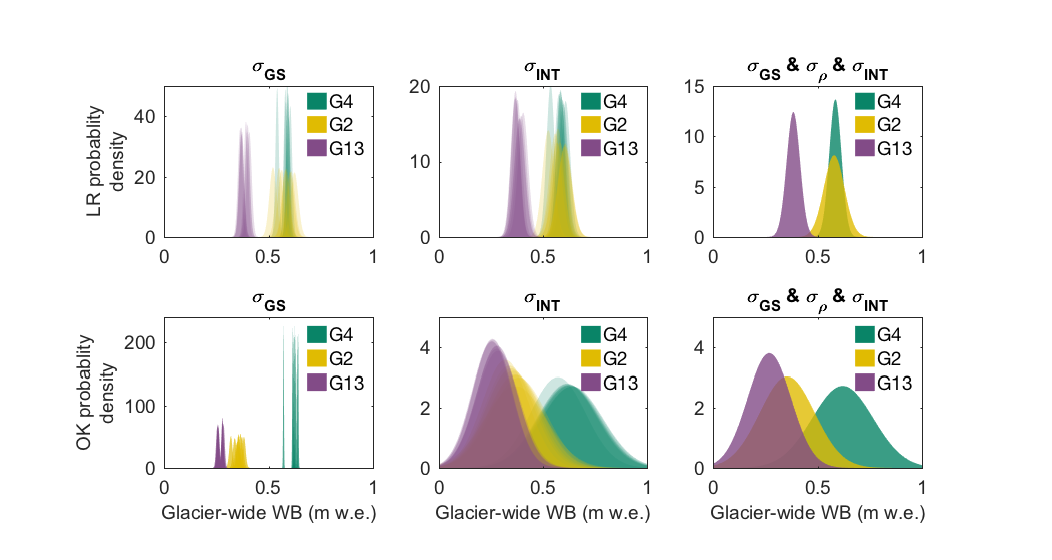
\includegraphics[width =0.95\textwidth]{WSMBDist.pdf}\\
%DIFDELCMD < 	%%%
%DIFDELCMD < \caption{%
{%DIFAUXCMD
\DIFdelFL{Distributions of glacier-wide winter balance (WB) for Glaciers 4 (G4), 2 (G2) and 13 (G13) that arise from various sources of uncertainty. WB distribution arising from grid-scale uncertainty ($\sigma_{\mathrm{GS}}$) (left column). WB distribution arising from interpolation uncertainty ($\sigma_{INT}$) (middle column). WB distribution arising from a combination of $\sigma_{\mathrm{GS}}$, $\sigma_{\mathrm{INT}}$ and density assignment uncertainty ($\sigma_{\rho}$) (right column). Results are shown for interpolation by linear regression (LR, top row) and simple kriging (SK, bottom row). Left two columns include eight distributions per glacier (colour) and each corresponds to a density assignment method (S1--S4 and F1--F4).}}
	%DIFAUXCMD
%DIFDELCMD < \label{fig:WSMBDist_LR}
%DIFDELCMD < \end{figure*}
%DIFDELCMD < %%%
\DIFdelend \DIFaddbegin \subsection{\DIFadd{Uncertainty analysis using a Monte Carlo approach}}
\DIFaddend 

\DIFdelbegin \subsection{\DIFdel{Uncertainty analysis}}
%DIFAUXCMD
\addtocounter{subsection}{-1}%DIFAUXCMD
%DIFDELCMD < 

%DIFDELCMD < %%%
\DIFdel{Glacier-wide winter balance is affected by uncertainty introduced by the representativeness of gridcell-averaged values of WB ($\sigma_{\mathrm{GS}}$), choosing a method of density assignment ($\sigma_{\rho}$), and interpolating WB values across the domain ($\sigma_{\mathrm{INT}}$). Using a Monte Carlo analysis, we find that interpolation uncertainty contributes more to WB uncertainty than grid-scale uncertainty or density assignment method. In other words, the distribution of glacier-wide WB that arises from grid-scale uncertainty and the differences in distributions between methods of density assignment are smaller than the distribution that arises from interpolation uncertainty (Fig. \ref{fig:WSMBDist_LR} and Table \ref{tab:WSMBdistribution_sigma}). The WB distributions obtained using LR and SK overlap for a given glacier, but the distribution modes differ (Fig. \ref{fig:WSMBDist_LR}). For reasons outlined above, SK-estimated values of WB in the accumulation area are generally lower, which lowers the glacier-wide WB estimate.  The uncertainty in SK-estimated values of WB is large, and unrealistic glacier-wide values of WB of 0\,m\,w.e. can be estimated (Fig. \ref{fig:WSMBDist_LR}). Our }\DIFdelend \DIFaddbegin \DIFadd{Interpolation/extrapolation of $b_\mathrm{w}$ data is the largest contributor of $B_\mathrm{w}$ uncertainty in our study. These }\DIFaddend results caution strongly against including \DIFdelbegin \DIFdel{extrapolated values of WB }\DIFdelend \DIFaddbegin \DIFadd{values of $B_\mathrm{w}$ }\DIFaddend in comparisons with remote sensing- or model-derived estimates of \DIFdelbegin \DIFdel{WB}\DIFdelend \DIFaddbegin \DIFadd{$B_\mathrm{w}$}\DIFaddend . If possible, such comparisons should be restricted to point-scale data. \DIFdelbegin %DIFDELCMD < 

%DIFDELCMD <  \begin{table*}[]
%DIFDELCMD < \centering
%DIFDELCMD < %%%
%DIFDELCMD < \caption{%
{%DIFAUXCMD
\DIFdelFL{Standard deviation ($\times10^{-2}$\,m\,w.e.) of glacier-wide winter balance distributions arising from uncertainties in grid-scale WB ($\sigma_{\mathrm{GS}}$), density assignment ($\sigma_{\rho}$), interpolation ($\sigma_{\mathrm{INT}}$) and all three sources combined ($\sigma_{\mathrm{ALL}}$) for linear regression (left columns) and simple kriging (right columns)}}
%DIFAUXCMD
%DIFDELCMD < \label{tab:WSMBdistribution_sigma}
%DIFDELCMD < \begin{tabular}{c|cccc|cccc}
%DIFDELCMD <  & \multicolumn{4}{c|}{\textbf{Linear regression}} & \multicolumn{4}{c}{\textbf{Simple kriging}} \\
%DIFDELCMD < %%%
\textbf{} %DIFAUXCMD
%DIFDELCMD < & %%%
\DIFdelFL{$\sigma_{\mathrm{GS}}$ }%DIFDELCMD < & %%%
\DIFdelFL{$\sigma_{\rho}$ }%DIFDELCMD < & %%%
\DIFdelFL{$\sigma_{INT}$ }%DIFDELCMD < & %%%
\DIFdelFL{$\sigma_{ALL}$ }%DIFDELCMD < & %%%
\DIFdelFL{$\sigma_{\mathrm{GS}}$ }%DIFDELCMD < & %%%
\DIFdelFL{$\sigma_{\rho}$ }%DIFDELCMD < & %%%
\DIFdelFL{$\sigma_{INT}$ }%DIFDELCMD < & %%%
\DIFdelFL{$\sigma_{ALL}$ }%DIFDELCMD < \\ \hline
%DIFDELCMD < %%%
\textbf{\DIFdelFL{Glacier 4}} %DIFAUXCMD
%DIFDELCMD < & %%%
\DIFdelFL{0.86 }%DIFDELCMD < & %%%
\DIFdelFL{1.90 }%DIFDELCMD < & %%%
\DIFdelFL{2.13 }%DIFDELCMD < & %%%
\DIFdelFL{2.90 }%DIFDELCMD < & %%%
\DIFdelFL{0.85 }%DIFDELCMD < & %%%
\DIFdelFL{2.15 }%DIFDELCMD < & %%%
\DIFdelFL{14.05 }%DIFDELCMD < & %%%
\DIFdelFL{14.72 }%DIFDELCMD < \\
%DIFDELCMD < %%%
\textbf{\DIFdelFL{Glacier 2}} %DIFAUXCMD
%DIFDELCMD < & %%%
\DIFdelFL{1.80 }%DIFDELCMD < & %%%
\DIFdelFL{3.37 }%DIFDELCMD < & %%%
\DIFdelFL{3.09 }%DIFDELCMD < & %%%
\DIFdelFL{4.90 }%DIFDELCMD < & %%%
\DIFdelFL{2.53 }%DIFDELCMD < & %%%
\DIFdelFL{2.03 }%DIFDELCMD < & %%%
\DIFdelFL{13.78 }%DIFDELCMD < & %%%
\DIFdelFL{13.44 }%DIFDELCMD < \\
%DIFDELCMD < %%%
\textbf{\DIFdelFL{Glacier 13}} %DIFAUXCMD
%DIFDELCMD < & %%%
\DIFdelFL{1.12 }%DIFDELCMD < & %%%
\DIFdelFL{1.68 }%DIFDELCMD < & %%%
\DIFdelFL{2.80 }%DIFDELCMD < & %%%
\DIFdelFL{3.20 }%DIFDELCMD < & %%%
\DIFdelFL{1.15 }%DIFDELCMD < & %%%
\DIFdelFL{1.27 }%DIFDELCMD < & %%%
\DIFdelFL{9.65 }%DIFDELCMD < & %%%
\DIFdelFL{10.43
}%DIFDELCMD < \end{tabular}
%DIFDELCMD < \end{table*}
%DIFDELCMD < 

%DIFDELCMD < %%%
\DIFdelend Grid-scale uncertainty ($\sigma_{\mathrm{GS}}$) is the smallest assessed contributor to overall \DIFdelbegin \DIFdel{WB }\DIFdelend \DIFaddbegin \DIFadd{$B_\mathrm{w}$ }\DIFaddend uncertainty. This result is consistent with the generally smoothly-varying snow depths encountered in zigzag surveys, and previously reported ice-roughness lengths on the order of centimetres \citep[e.g.][]{Hock2005} compared to snow depths on the order of decimetres to metres. Given our assumption that zigzags are an adequate representation of grid-scale variability, the low \DIFdelbegin \DIFdel{WB }\DIFdelend \DIFaddbegin \DIFadd{$B_\mathrm{w}$ }\DIFaddend uncertainty arising from $\sigma_{\mathrm{GS}}$ implies that subgrid-scale sampling need not be a high priority for reducing overall uncertainty. Our assumption that the 3--4 zigzag surveys can be used to estimate glacier-wide $\sigma_{\mathrm{GS}}$ may be flawed, particularly in areas with debris cover, crevasses and steep slopes.

Our analysis did not include uncertainty arising from \DIFdelbegin \DIFdel{a number of sources, which we assume either to be  encompassed by the sources investigated or to be negligible contributors. These sources of uncertainty include }\DIFdelend density measurement errors associated with the \DIFdelbegin \DIFdel{Federal Sampler}\DIFdelend \DIFaddbegin \DIFadd{FS}\DIFaddend , wedge cutters and spring scales, \DIFaddbegin \DIFadd{from }\DIFaddend vertical and horizontal errors in the DEM \DIFdelbegin \DIFdel{and }\DIFdelend \DIFaddbegin \DIFadd{or from }\DIFaddend error associated with estimating measurement locations \DIFdelbegin \DIFdel{.
}%DIFDELCMD < 

%DIFDELCMD < %%%
\DIFdel{The values of glacier-wide WB for our study glaciers (using LR and S2 density assignment method), with an uncertainty equal to one standard deviation of the distribution found with Monte Carlo analysis, are: 0.59\,$\pm$\,0.03\,m\,w. e. for Glacier 4, 0.61\,$\pm$\,0.05\,m\,w.e. for Glacier 2 and 0.40\,$\pm$\,0.03\,m\,w.e. for Glacier 13. The glacier-wide WB uncertainty from combined }\DIFdelend \DIFaddbegin \DIFadd{based on the GPS position of the lead observer. We assume that these }\DIFaddend sources of uncertainty \DIFdelbegin \DIFdel{ranges from 0.03\,m w.
e (5\%) to 0.05\,m w.e (8\%) for linear-regression estimates and from 0.10\,m w.e (37\%) to 0.15\,m w.e (24\%) for simple-kriging estimates (Table \ref{tab:WSMB&RMSE}).
}\DIFdelend \DIFaddbegin \DIFadd{are either encompassed by the sources investigated or are negligible.
}\DIFaddend 


\subsection{\DIFdelbegin \DIFdel{Context and caveats}\DIFdelend \DIFaddbegin \DIFadd{Regional winter-balance gradient}\DIFaddend }
\DIFdelbegin \subsubsection{\DIFdel{Regional winter-balance gradient}}
%DIFAUXCMD
\addtocounter{subsubsection}{-1}%DIFAUXCMD
\DIFdelend 

Although we find considerable inter- and intra-basin variability in winter balance, our results are consistent with a regional-scale winter-balance gradient for the continental side of the St. Elias Mountains (Fig. \ref{fig:AccumGrad}). Winter-balance data are compiled from \cite{Taylor1969}, the three glaciers presented in this paper and two \DIFdelbegin \DIFdel{snow pits }\DIFdelend \DIFaddbegin \DIFadd{SP }\DIFaddend we analyzed near the head of the Kaskawulsh Glacier between 20--21 May 2016. The data show a linear decrease of $0.024$\,m\,w.e. km$^{-1}$ (R$^2=0.85$) in winter balance with distance from the regional topographic divide between the Kaskawulsh and Hubbard Glaciers, as identified by \cite{Taylor1969}. While the three study glaciers fit the regional trend, the same relationship would not apply if just the Donjek Range were considered. We hypothesize that interaction between meso-scale weather patterns and large-scale mountain topography is a major driver of regional-scale winter balance. Further insight into regional-scale patterns of winter balance in the St. Elias Mountains could be gained by investigating moisture source trajectories and the contribution of orographic precipitation. 

\begin{figure}
	\centering
	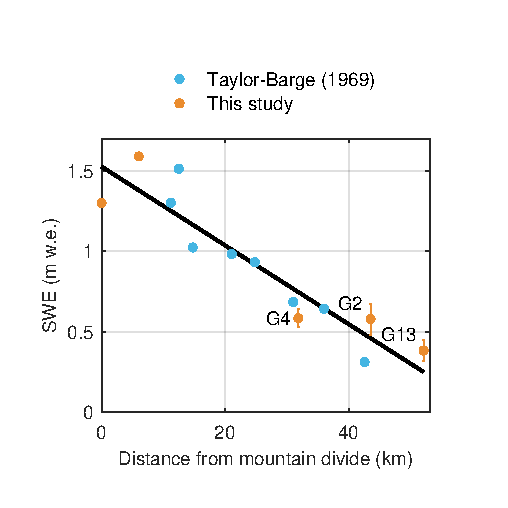
\includegraphics[width =0.35\textwidth]{AccumGrad.pdf}\\
	\caption{Relationship between winter balance \DIFdelbeginFL \DIFdelFL{(WB) }\DIFdelendFL and linear distance from the regional topographic divide between the Kaskawulsh and Hubbard Glaciers in the St. Elias Mountains. Point-scale values of \DIFdelbeginFL \DIFdelFL{WB }\DIFdelendFL \DIFaddbeginFL \DIFaddFL{winter balance }\DIFaddendFL from snow-pit data reported by \cite{Taylor1969} (blue boxes, P-WB). LR-estimated glacier-wide \DIFdelbeginFL \DIFdelFL{WB }\DIFdelendFL \DIFaddbeginFL \DIFaddFL{winter balance ($B_\mathrm{w}$) }\DIFaddendFL calculated using density assignment S2 for Glaciers 4 (G4), 2 (G2) and 13 (G13) with errors bars calculated as the standard deviation of Monte Carlo-derived \DIFdelbeginFL \DIFdelFL{WB }\DIFdelendFL \DIFaddbeginFL \DIFaddFL{$B_\mathrm{w}$ }\DIFaddendFL distributions (this study) (open orange circles, G-WB). Point-scale \DIFdelbeginFL \DIFdelFL{WB }\DIFdelendFL \DIFaddbeginFL \DIFaddFL{winter balance }\DIFaddendFL estimated from snow-pit data at two locations in the accumulation area of the Kaskawulsh Glacier, collected in May 2016 (unpublished data, SFU Glaciology Group) (filled orange dots, P-WB). Black line indicates best fit (R$^2=0.85$).}
	\label{fig:AccumGrad}
\end{figure}

\DIFdelbegin \subsubsection{\DIFdel{Limitations and future work}}
%DIFAUXCMD
\addtocounter{subsubsection}{-1}%DIFAUXCMD
\DIFdelend \DIFaddbegin \subsection{\DIFadd{Limitations and future work}}
\DIFaddend 

The potential limitations of our work include the restriction of our data to a single year, minimal sampling in the accumulation area, the problem of uncorrelated SP- and FS-derived densities, a sampling design that could not be optimized \DIFdelbegin \DIFdel{a priori}\DIFdelend \DIFaddbegin \textit{\DIFadd{a priori}}\DIFaddend , the assumption of spatially uniform subgrid variability and lack of more finely resolved DEMs.

Inter-annual variability in winter balance is not considered in our study. A number of studies have found temporal stability in spatial patterns of snow distribution and that statistical models based on topographic parameters could be applied reliably between years \citep[e.g.][]{Grunewald2013}. For example, \cite{Walmsley2015} analyzed more than 40 years of winter balance recorded on two Norwegian glaciers and found that snow distribution is spatially heterogeneous yet exhibits robust temporal stability. Contrary to this, \cite{Crochet2007} found that snow distribution in Iceland differed considerably between years and depended primarily on the dominant wind direction over the course of a winter. Therefore, multiple years of snow depth and density measurements, that are not necessarily consecutive, are needed to better understand inter-annual variability \DIFdelbegin \DIFdel{in winter-balance distribution }\DIFdelend \DIFaddbegin \DIFadd{of winter balance }\DIFaddend within the Donjek Range.

There is a conspicuous lack of data in the accumulation areas of our study glaciers. With increased sampling in the accumulation area, interpolation uncertainties would be reduced where they are currently greatest and the \DIFdelbegin \DIFdel{linear regression }\DIFdelend \DIFaddbegin \DIFadd{LR }\DIFaddend would be better constrained. Although certain regions of the glaciers remain inaccessible for direct measurements, other methods of obtaining winter-balance \DIFaddbegin \DIFadd{measurements}\DIFaddend , including ground-penetrating radar and DEM differencing with photogrammetry or lidar, could be used in conjunction with manual probing to increase the spatial coverage of measurements.

The lack of correlation between SP- and FS-derived densities needs to be reconciled. Contrary to our results, most studies that compare SP- and FS-derived densities report minimal discrepancy \citep[e.g.][and sources within]{Dixon2012}. Additional co-located density measurements are needed to better compare the two methods of obtaining density values. Comparison with other \DIFdelbegin \DIFdel{Federal Samplers }\DIFdelend \DIFaddbegin \DIFadd{FS }\DIFaddend would also be informative. Even with this limitation, density assignment was, fortunately, not the largest source of uncertainty in estimating glacier-wide winter balance. 

Our sampling design was chosen to achieve broad spatial coverage of the ablation area, but is likely too finely resolved along transects for many mass-balance surveys to replicate. An optimal sampling design would minimize uncertainty in winter balance while reducing the number of required measurements. Analysis of the estimated winter balance obtained using subsets of the data is underway to make recommendations on optimal transect configuration and along-track spacing of measurements. \cite{Lopez2010} found that 200--400 observations are needed within a non-glacierized alpine basin (6\,km$^2$) to obtain accurate and robust snow distribution models. Similar guidelines would be useful for glacierized environments.

In this study, we assume that the subgrid variability of winter balance is uniform across a given glacier. Contrary to this assumption, \cite{McGrath2015} found greater variability of winter-balance values close to the terminus. Testing our assumption could be a simple matter of prioritizing the labour-intensive zigzags surveys. To ensure consistent quantification of subgrid variability, zigzag survey measurements could also be tested against other measurements methods, such as lidar. 

DEM gridcell size is known to influence values of computed topographic parameters \citep{Zhang1994, Garbrecht1994, Guo-an2001, Lopez2010}. The relationship between topographic parameters and winter balance is, therefore, not independent of DEM gridcell size. For example, \cite{Kienzle2004} and \cite{Lopez2010} found that a decrease in spatial resolution of the DEM results in a decrease in the importance of curvature and an increase in the importance of elevation in \DIFdelbegin \DIFdel{regressions }\DIFdelend \DIFaddbegin \DIFadd{LR }\DIFaddend of snow distribution on topographic parameters in non-glacierized basins. The importance of curvature in our study is affected by the DEM smoothing that we applied to obtain a spatially continuous curvature field (see Supplementary Material\DIFaddbegin \DIFadd{, Fig. S1}\DIFaddend ). A comparison of regression coefficients from high-resolution DEMs obtained from various sources and sampled with various gridcell sizes could be used to characterize the dependence of topographic parameters on DEMs, and therefore assess the robustness of inferred relationships between winter balance and topographic parameters. 


%%%%%%%%%%%%%%%%%%%%%%%%%%%%%%%%%%
% CONCLUSION
%%%%%%%%%%%%%%%%%%%%%%%%%%%%%%%%%%
\section{Conclusion}

We estimate winter balance for three glaciers (termed Glacier 2, Glacier 4 and Glacier 13) in the St. Elias Mountains, Yukon, Canada from multiscale snow depth and density measurements. Linear regression and \DIFdelbegin \DIFdel{simple }\DIFdelend \DIFaddbegin \DIFadd{ordinary }\DIFaddend kriging are used to obtain estimates of distributed winter balance \DIFaddbegin \DIFadd{($b_\mathrm{w}$)}\DIFaddend . We use Monte Carlo analysis to evaluate the contributions of interpolation, \DIFdelbegin \DIFdel{the }\DIFdelend assignment of snow density and grid-scale variability of winter balance to uncertainty in \DIFaddbegin \DIFadd{estimates of }\DIFaddend glacier-wide winter balance \DIFaddbegin \DIFadd{($B_\mathrm{w}$)}\DIFaddend . 

Values of \DIFdelbegin \DIFdel{glacier-wide winter balance }\DIFdelend \DIFaddbegin \DIFadd{$B_\mathrm{w}$ }\DIFaddend estimated using linear regression and \DIFdelbegin \DIFdel{simple }\DIFdelend \DIFaddbegin \DIFadd{ordinary }\DIFaddend kriging differ by up to 0.24\,m\,w.e. ($\sim$50\%). We find that interpolation uncertainty is the largest assessed source of uncertainty in \DIFdelbegin \DIFdel{glacier-wide winter balance (5}\DIFdelend \DIFaddbegin \DIFadd{$B_\mathrm{w}$ (7}\DIFaddend \% for linear-regression estimates and \DIFdelbegin \DIFdel{32\% for simple-kriging }\DIFdelend \DIFaddbegin \DIFadd{34\% for ordinary-kriging }\DIFaddend estimates). Uncertainty resulting from the method of density assignment is comparatively low, despite the wide range of methods explored. Given our representation of grid-scale variability, the resulting \DIFdelbegin \DIFdel{winter balance }\DIFdelend \DIFaddbegin \DIFadd{$B_\mathrm{w}$ }\DIFaddend uncertainty is small indicating that extensive subgrid-scale sampling is not required to reduce overall uncertainty. 

Our results suggest that processes governing distributed \DIFdelbegin \DIFdel{winter balance }\DIFdelend \DIFaddbegin \DIFadd{$b_\mathrm{w}$ }\DIFaddend differ between glaciers, highlighting the importance of regional-scale winter-balance studies. The estimated distribution of \DIFdelbegin \DIFdel{winter balance }\DIFdelend \DIFaddbegin \DIFadd{$b_\mathrm{w}$ }\DIFaddend on Glacier 4 is characterized by high variability, as indicated by the poor correlation between estimated and observed values and large number of data outliers. Glaciers 2 and 13 appear to have lower spatial variability, with elevation being the dominant predictor of gridcell-averaged \DIFdelbegin \DIFdel{winter balance}\DIFdelend \DIFaddbegin \DIFadd{$b_\mathrm{w}$}\DIFaddend . A wind-redistribution parameter is found to be a weak but significant predictor of \DIFdelbegin \DIFdel{winter balance}\DIFdelend \DIFaddbegin \DIFadd{$b_\mathrm{w}$}\DIFaddend , though conflicting relationships between glaciers make it difficult to interpret. \DIFaddbegin \DIFadd{The major limitations of our work include the restriction of our data to a single year and minimal sampling in the accumulation area. }\DIFaddend Although challenges persist when estimating winter balance, our data are consistent with a regional-scale winter-balance gradient for the continental side of the St. Elias Mountains. 

\section{Author contribution statement}

AP planned and executed the data collection, performed all calculations and drafted the manuscript. GF conceived of the study, contributed to field planning and data collection, oversaw all stages of the work and edited the manuscript. VR provided guidance with statistical methods and edited the manuscript.

\section{Acknowledgements}

We thank the Kluane First Nation (KFN), Parks Canada and the Yukon Territorial Government for granting us permission to work in KFN Traditional Territory and Kluane National Park and Reserve. We are grateful for financial support provided by the Natural Sciences and Engineering Research Council of  Canada, Simon Fraser University and the Northern Scientific  Training  Program. We kindly acknowledge Kluane Lake Research Station, Sian Williams, Lance Goodwin and Trans North pilot Dion Parker for facilitating field logistics. We are grateful to Alison Criscitiello and Coline Ariagno for all aspects of field assistance and Sarah Furney for assistance with data entry. Thank you to Etienne Berthier for providing us with the SPIRIT SPOT-5 DEM and for assistance in DEM correction. We are grateful to Derek Bingham and Michael Grosskopf for assistance with the statistics, including \DIFdelbegin \DIFdel{simple }\DIFdelend \DIFaddbegin \DIFadd{ordinary }\DIFaddend kriging. Luke Wonneck, Leif Anderson and Jeff Crompton all provided thoughtful and constructive comments on drafts of the manuscript.


%----------------------------------------------------------------------------------------
%	REFERENCE LIST
%----------------------------------------------------------------------------------------
%
%\bibliography{MastersLit}
%\bibliography{/home/glaciology1/Documents/MastersDocuments/MastersLit}
\bibliography{/Users/Alexandra/Documents/SFU/MastersDocuments/MastersLit}
\bibliographystyle{igs}

%----------------------------------------------------------------------------------------


\end{document}

